% Created 2017-06-05 Mon 11:42
\documentclass[9pt,lineo]{elife}

\usepackage{amsmath}
\usepackage{amssymb}
\usepackage[version=4]{mhchem}
\usepackage{siunitx}


              \usepackage[utf8]{inputenc}
\sisetup{detect-all}
\author[1]{David R. Hill}
\corr{spencejr@umich.edu}{JRS}
\corr{youngvi@umich.edu}{VBY}
\author[1]{Sha Huang}
\author[2]{Courtney Fields}
\author[3]{Dishari Mukherjee}
\author[2]{Brooke Bons}
\author[1]{Shrikar Thodla}
\author[4]{Priya H. Dedhia}
\author[1]{Alana M. Chin}
\author[1]{Yu-Hwai Tsai}
\author[1]{Melinda S. Nagy}
\author[3]{Thomas M. Schmidt}
\author[6]{Seth Walk}
\author[1,2,3\authfn{1}]{Vincent B. Young}
\author[1,5\authfn{1}]{and Jason R. Spence}
\affil[1]{Department of Internal Medicine, Division of Gastroenterology, University of Michigan, Ann Arbor MI 48109}
\affil[2]{Department of Internal Medicine, Division of Infectious Disease, University of Michigan, Ann Arbor MI 48109}
\affil[3]{Department of Microbiology and Immunology, University of Michigan, Ann Arbor MI 48109}
\affil[4]{Department of Surgery,University of Michigan, Ann Arbor MI 48109}
\affil[5]{Department of Cell and Developmental Biology, University of Michigan, Ann Arbor MI 48109}
\affil[6]{Department of Microbiology and Immunology, Montana State University, Bozeman, MT 59717}
\contrib[\authfn{1}]{These authors contributed equally to this work}
\setcounter{secnumdepth}{0}
\date{\today}
\title{Bacterial colonization stimulates a complex physiological response in the immature human intestinal epithelium}
\begin{document}

\maketitle
\begin{abstract}

The human gastrointestinal tract is immature at birth, yet must adapt to dramatic changes such as oral nutrition and microbial colonization. The confluence of these factors can lead to severe inflammatory disease in premature infants; however, investigating complex environment-host interactions is difficult due to limited access to immature human tissue. Here, we demonstrate that the epithelium of human pluripotent stem cell-derived human intestinal organoids is globally similar to the immature human epithelium and we utilize HIOs to investigate complex host-microbe interactions in this na{\"i}ve epithelium.  Our findings demonstrate that the immature epithelium is intrinsically capable of establishing a stable host-microbe symbiosis. Microbial colonization leads to complex contact and hypoxia driven responses resulting in increased antimicrobial peptide production, maturation of the mucus layer, and improved barrier function. These studies lay the groundwork for an improved mechanistic understanding of how colonization influences development of the immature human intestine. 
\end{abstract}

\section*{{\bfseries\sffamily } Introduction}
\label{sec:orgheadline1}
The epithelium of the gastrointestinal (GI) tract represents a large surface area for host-microbe interaction and mediates the balance between tolerance of mutualistic organisms and the exclusion of potential pathogens \citep{Peterson:2014}. This is accomplished, in part, through the formation of a tight physical epithelial barrier, in addition to epithelial secretion of anti-microbial peptides and mucus \citep{Veereman-Wauters:1996,Renz:2012}. Development and maturation of the epithelial barrier coincides with the first exposure of the GI tract to microorganisms and the establishment of a microbial community within the gut \citep{Palmer:2007,Koenig:2011}. Although microorganisms have long been appreciated as the primary drivers of the postnatal expansion of adaptive immunity \citep{Renz:2012,Shaw:2010,Hviid:2011,Abrahamsson:2014,Arrieta:2015}, and more recently as key stimuli in the development of digestion \citep{Erkosar:2015}, metabolism \citep{Cho:2012}, and neurocognitive function \citep{Diaz_Heijtz:2011,Clarke:2014,Borre:2014,Desbonnet:2014}, it remains unclear how the human epithelial surface adapts to colonization and expansion of microorganisms within the immature GI tract.

Studies in gnotobiotic mice have improved our understanding of the importance of microbes in normal gut function since these mice exhibit profound developmental defects in the intestine \citep{Round:2009,Gensollen:2016,Bry:1996,Hooper:1999} including decreased epithelial turnover, impaired formation of microvilli \citep{ABRAMS:1963}, and altered mucus glycosylation at the epithelial surface \citep{Bry:1996,Goto:2014,Cash:2006}. However, evidence also suggests that the immature human intestine may differ significantly from the murine intestine, especially in the context of disease \citep{Nguyen:2015}. For example, premature infants can develop necrotizing enterocolitis (NEC), an inflammatory disease with unknown causes. Recent reports suggest a multifactorial etiology by which immature intestinal barrier function predisposes the preterm infant to intestinal injury and inflammation following postpartum microbial colonization \citep{Neu:2011,Morrow:2013,Greenwood:2014,Hackam:2013,Afrazi:2014,Fusunyan:2001,Nanthakumar:2011}. Rodent models of NEC have proven to be inadequate surrogates for studying human disease \citep{Tanner:2015}. Therefore, direct studies of host-microbial interactions in the immature human intestine will be important to understand the complex interactions during bacterial colonization that lead to a normal gut development or disease.

Important ethical and practical considerations have limited research on the immature human intestine. For example, neonatal surgical specimens are often severely damaged by disease and not conducive for \emph{ex vivo} studies. We and others have previously demonstrated that human pluripotent stem cell derived human intestinal organoids (HIOs) closely resemble immature intestinal tissue \citep{Spence:2011,Finkbeiner:2015,Watson:2014,Forster:2014,Dedhia:2016,Aurora:2016,Chin:2017} and recent work has established gastrointestinal organoids as a powerful model of microbial pathogenesis at the mucosal interface \citep{Leslie:2015,McCracken:2014,Forbester:2015, Hill:2017}. 

In the current work, we used HIOs as a model immature intestinal epithelium and a human-derived non-pathogenic strain of \emph{E. coli} as a model intestinal colonizer to examine how host-microbe interactions affected intestinal maturation and function.  Although the composition of the neonatal intestinal microbiome varies between individuals, organisms within the genera \emph{Escherichia} are dominant early colonizers \citep{Gosalbes:2013,Backhed:2015} and commensal \emph{E. coli} are widely prevalent and highly abundant components of the neonatal stool microbiome \citep{Palmer:2007,Koenig:2011,Backhed:2015,Morrow:2013}. Microinjection of \emph{E. coli} into the lumen of 3-dimensional HIOs resulted in stable bacterial colonization \emph{in vitro}, and using RNA-sequencing, we monitored the global transcriptional changes in response to colonization. We observed widespread, time-dependent transcriptional responses that are the result of both bacterial contact and luminal hypoxia resulting from bacterial colonization in the HIO. Bacterial association with the immature epithelium increased antimicrobial defenses and resulted in enhanced epithelial barrier function and integrity. We observed that NF-\(\kappa\)B is a central downstream mediator of the transcriptional changes induced by both bacterial contact and hypoxia. We further probed the bacterial contact and hypoxia dependent epithelial responses using experimental hypoxia and pharmacological NF-\(\kappa\)B inhibition, which allowed us to delineate which of the transcriptional and functional responses of the immature epithelium were oxygen and/or NF-\(\kappa\)B dependent. We found that NF-\(\kappa\)B dependent microbe-epithelial interactions were beneficial by enhancing barrier function and protecting the epithelium from damage by inflammatory cytokines.  Collectively, these studies shed light on how microbial contact with the immature human intestinal epithelium can lead to modified function.

\section*{{\bfseries\sffamily } Results}
\label{sec:orgheadline10}

\subsection*{{\bfseries\sffamily } Pluripotent stem-cell derived intestinal epithelium transcriptionally resembles the immature human intestinal epithelium}
\label{sec:orgheadline2}
Previous work has demonstrated that stem cell derived human intestinal organoids resemble immature human duodenum \citep{Watson:2014,Finkbeiner:2015,Tsai:2017}. Moreover, transplantation into immunocompromised mice results in HIO maturation to an adult-like state \citep{Watson:2014,Finkbeiner:2015}. These analyses compared HIOs consisting of epithelium and mesenchyme to whole-thickness human intestinal tissue, which also possessed cellular constituents lacking in HIOs such as neurons, blood vessels and immune cells  \citep{Finkbeiner:2015}. Thus the extent to which the HIO epithelium resembles immature/fetal intestinal epithelium remains unclear. To address this gap and further characterize the HIO epithelium relative to fetal and adult duodenal epithelium, we isolated and cultured epithelium from HIOs grown entirely \emph{in vitro}, from fetal duodenum, adult duodenum, or HIOs that had been transplanted into the kidney capsule of NSG immuno-deficient mice and matured for 10 weeks. These epithelium-only derived organoids were expanded \emph{in vitro} in uniform tissue culture conditions for 4-5 passages and processed for RNA-sequencing (RNA-seq) (\textbf{Figure 1 - Supplement 1}). Comparison of global transcriptomes between all samples in addition to human embryonic stem cells (hESCs) used to generate HIOs (\citealt{Finkbeiner:2015}; E-MTAB-3158) revealed a clear hierarchy in which both \emph{in vitro} grown HIO epithelium (\emph{P} = \num{5.06e-9}) and transplanted epithelium (\emph{P} = \num{7.79e-14}) shares a substantially greater degree of similarity to fetal small intestinal epithelium (\textbf{Figure 1 - Supplement 1A}). 

While unbiased clustering demonstrated that transplanted epithelium is closely resembles fetal epithelium, we noted a shift towards the adult transcriptome that resulted in a relative increase in the correlation between transplanted HIO epithelium and adult duodenum-derived epithelium grown \emph{in vitro}  (\textbf{Figure 1 - Supplement 1B}, \emph{P} = \num{1.17e-4}). Principle component analysis (PCA) of this multi-dimensional gene expression dataset (\textbf{Figure 1 - Supplement 1C}) corroborated the correlation analysis, and indicated that developmental stage  (PC1, 27.75\% cumulative variance) and tissue maturation status (PC2, 21.49\% cumulative variance) were major drivers accounting for a total of 49.24\% of the cumulative variance between samples. Here, HIO epithelium clustered with fetal epithelium along PC2 whereas transplanted HIO epithelium clustered with adult epithelium.

We further used differential expression analysis to demonstrate that in vitro grown HIO epithelium is similar to the immature human intestine whereas \emph{in vivo} transplanted HIO epithelium is similar to the adult epithelium.  To do this, we identified differentially expressed genes through two independent comparisons: 1) human fetal vs. adult epithelium; 2) HIO epithelium vs. transplanted HIO epithelium. Genes enriched in transplanted HIO epithelium relative to the HIO epithelium were compared to genes enriched in the adult duodenum relative to fetal duodenum (\textbf{Figure 1 - Supplement 1D}). There was a highly significant correlation between log\(_{\text{2}}\)-transformed expression ratios where transplanted HIOs and adult epithelium shared enriched genes while HIO and fetal epithelium shared enriched genes  (\emph{P} = \num{2.6e-28}). This analysis supports previously published data indicating that the epithelium from HIOs grown \emph{in vitro} recapitulates the gene expression signature of the immature duodenum and demonstrates that the HIO epithelium is capable of adopting a transcriptional signature that more strongly resembles adult duodenum following transplantation into mice.

\subsection*{{\bfseries\sffamily } HIOs can be stably associated with commensal \emph{E. coli}}
\label{sec:orgheadline3}
Given that the HIO epithelium recapitulates many of the features of the immature intestinal epithelium, we set out to evaluate the effect of bacterial colonization on the na{\"i}ve HIO epithelium. Previous studies have established that pluripotent stem cell derived intestinal organoids can be injected with live viral \citep{Finkbeiner:2012} or bacterial pathogens \citep{Leslie:2015,Engevik:2015,Forbester:2015}, however it was not known if HIOs could be stably co-cultured with non-pathogenic or commensal microorganisms. We co-cultured HIOs with the human commensal microbe \emph{Esherichia coli} strain ECOR2 \citep{Ochman:1984} using a microinjection technique to introduce live \emph{E. coli} into the HIO lumen in a manner that prevented contamination of the surrounding media. HIOs microinjected with \num{e5} live \emph{E. coli} constitutively expressing GFP exhibit robust green fluorescence within 3 h of microinjection (\textbf{Figure 1A} and \textbf{Supplementary File 1}). Numerous E. coli localized to the luminal space at 48 h post-microinjection and are present adjacent to the HIO epithelium, with some apparently residing in close opposition to the apical epithelial surface (\textbf{Figure 1B}).

In order to determine the minimum number of CFU \emph{E. coli} required to establish short term colonization (24 hours), we microinjected increasing concentrations of live \emph{E. coli} suspended in PBS into single HIOs and collected and enumerated bacteria in the luminal contents at 24 h post-microinjection (\textbf{Figure 1C}). Single HIOs can be stably colonized by as few as 5 CFU \emph{E. coli} per HIO with 77.8 \% success (positive luminal culture and negative external media culture at 24 h post-injection) and 100 \% success at \(\ge\) 100 CFU per HIO (\textbf{Figure 1C}).  Increasing the number of CFU \emph{E. coli} microinjected into each HIO at \emph{t} = 0 did not increase the mean luminal CFU per HIO at 24 hours post-microinjection (\emph{P} = 0.37; \textbf{Figure 1C}). Thus, the 24 h growth rate of \emph{E. coli} within the HIO lumen was negatively correlated with the CFU injected (R\(^{\text{2}}\) = 0.625, P = \num{3.1e-12}; \textbf{Figure 1C}). 

Next, we examined the stability of HIO and commensal \emph{E. coli} co-cultures over time \emph{in vitro}. HIOs were microinjected with 10 CFU \emph{E. coli} and maintained for 24-72 h (\textbf{Figure 1D}). Rapid expansion of \emph{E. coli} density within the HIO lumen was observed in the first 24 h, with relatively stable bacterial density at 48-72 hr. A 6.25-fold increase in bacterial density was observed between 24 and 72 h post-microinjection (\emph{P} = 0.036). Importantly, samples taken from the external HIO culture media were negative for \emph{E. coli} growth under all microinjection conditions (\textbf{Figure 1E}).

Finally, we examined the stability of HIO cultures following \emph{E. coli} microinjection (\textbf{Figure 1F}). A total of 48 individual HIOs were microinjected with 10\(^{\text{4}}\) CFU \emph{E. coli} each. Controls were microinjected with sterile PBS alone. The external HIO media was sampled daily and cultured for bacterial growth. External culture media was sterile in 100\% of control HIOs throughout the entire experiment, and in 100 \% of \emph{E. coli} injected HIOs on days 0-2 post-microinjection. On days 3-9 post-microinjection some cultured media was positive for \emph{E. coli} growth; however, 77.08 \% of \emph{E. coli} injected HIOs were negative for \emph{E. coli} in the external culture media throughout the timecourse. Thus, the large majority of \emph{E. coli} colonized HIOs remain stable for an extended period when cultured \emph{in vitro} and without antibiotics.

\begin{figure}
\begin{fullwidth}
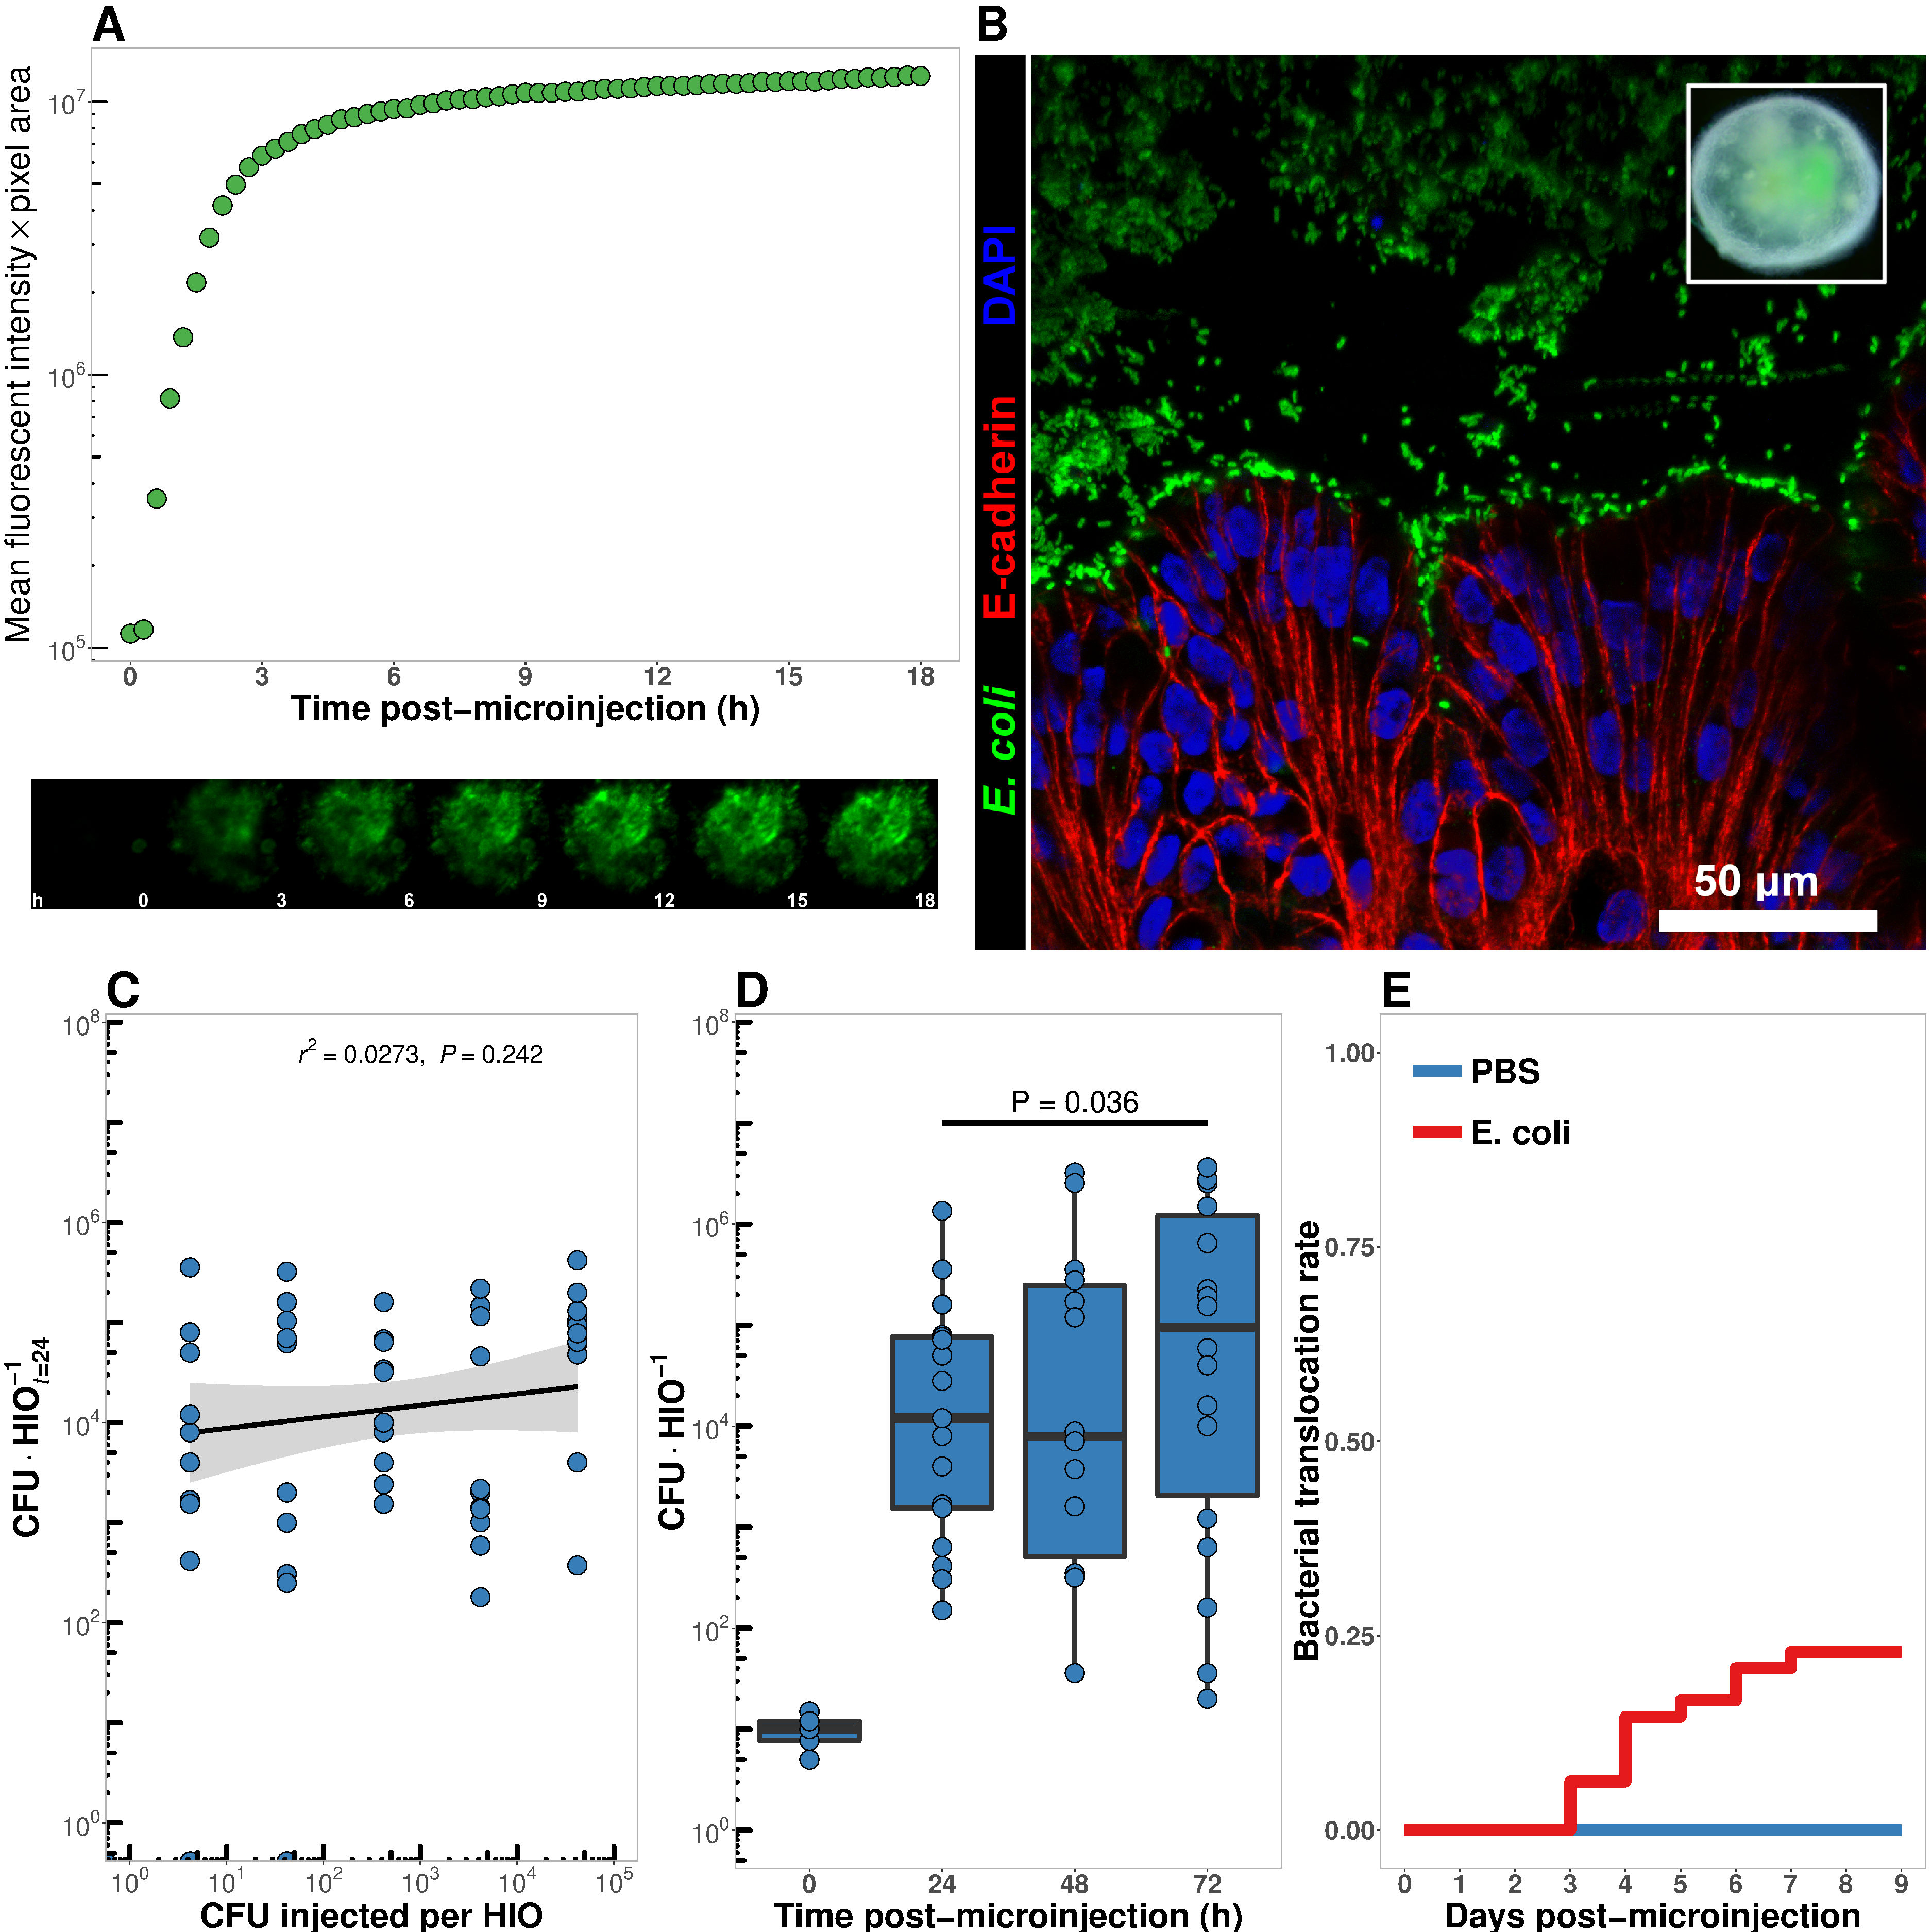
\includegraphics[width=0.95\linewidth]{./figures/figure1/figure1_multipanel.pdf}
\caption{\textbf{A} Human intestinal organoid (HIO) containing live GFP+ \textit{E. coli} str. ECOR2. Brightfield, fluorescent, and overlay images are labeled. \textbf{B} Confocal micrograph of the HIO epithelium (E-cadherin) in direct association with GFP+ \textit{E. coli}. \textbf{C} Luminal CFU per HIO \textit{E. coli} at 24 h post-microinjection with \numrange{5e-1}{5e5} CFU per HIO. \textbf{D} Luminal CFU per HIO at 0-72 h post microinjection. \textbf{E} HIO culture media or HIO luminal contents plated on LB agar and cultured overnight at \SI{37}{\celsius}. \textbf{F} Daily proportion of HIO cultures with no culturable \textit{E. coli} in the external media following \textit{E. coli} microinjection (n = 48) or PBS microinjection (n = 8).}
\label{fig:fullwidth}
\end{fullwidth}
\end{figure}

\subsection*{{\bfseries\sffamily } Bacterial association elicits a broad-scale, time-dependent transcriptional response}
\label{sec:orgheadline4}
Colonization of the immature gut by microbes is associated with functional maturation in both model systems\citep{Kremer:2013,Sommer:2015,Broderick:2014,Erkosar:2015} and in human infants \citep{Renz:2012}. To evaluate if exposing HIOs to \emph{E. coli} led to maturation at the epithelial interface, we evaluated the transcriptional events following microinjection of live \emph{E. coli}  into the HIO lumen. PBS-injected HIOs (controls) and HIOs co-cultured with \emph{E. coli} were collected for RNA-seq after 24, 48 and 96 hours (\textbf{Figure 2}). At 24 h post-microinjection, a total of 2,018 genes were differentially expressed (adjusted-FDR < 0.05), and the total number of differentially expressed was further increased at 48 and 96 h post-microinjection relative to PBS-injected controls (\textbf{Figure 2A}). Principle component analysis demonstrated that global transcriptional activity in HIOs is significantly altered by exposure to E. coli, with the degree of transcriptional changes relative to control HIOs increasing over time (\textbf{Figure 2B}).

Gene set enrichment analysis (GSEA) \citep{Subramanian:2005} using the GO \citep{Ashburner:2000,Gene_Ontology_Consortium:2015} and REACTOME \citep{Croft:2014,Fabregat:2016} databases to evaluate RNA-seq expression data revealed coordinated changes in gene expression related to innate anti-microbial defense, epithelial barrier production, adaptation to low oxygen, and tissue maturation (\textbf{Figure 2C}). Innate anti-microbial defense pathways, including genes related to NF-\(\kappa\)B signaling, cytokine production, and Toll-like receptor (TLR) signaling were strongly up-regulated at 24 h post-microinjection and generally exhibited decreased activation at later time points. GSEA also revealed changes in gene expression consistent with reduced oxygen levels or hypoxia, including the induction of pro-angiogenesis signals. A number of pathways related to glycoprotein synthesis and modification, including O-linked mucins, glycosaminoglycans, and proteoglycans, were up-regulated in the initial stages of the transcriptional response (Syndecans, integrins), exhibited a somewhat delayed onset (O-linked mucins), or exhibited consistent activation at all time points post-microinjection (Keratan sulfate and glycosaminoglycan biosynthesis). Finally, genes sets associated with a range of processes involved in tissue maturation and development followed a distinct late-onset pattern of expression. This included broad gene ontology terms for organ morphogenesis, developmental maturation, and regionalization as well as more specific processes such as differentiation of mesenchymal and muscle cells, and processes associated with the nervous system (\textbf{Figure 2C}).

We also made correlations between upregulated genes in the RNA-seq data (\textbf{Figure 2D}) and protein factors present in the organoid culture media following \emph{E. coli} microinjection (\textbf{Figure 2E}). \(\beta\)-defensin 1 (\emph{DEFB1} (gene); BD-1 (protein)) and \(\beta\)-defensin 2 (\emph{DEFB4A} (gene); BD-2 (protein)) exhibited distinct patterns of expression, with both \emph{DEFB1} and its protein product BD-1 stable at 24 hours after \emph{E. coli} microinjection but relatively suppressed at later time points, and \emph{DEFB4A} and BD-2 strongly induced at early time points and subsiding over time relative to PBS-injected controls. By contrast, inflammatory regulators IL-6 and IL-8 and the pro-angiogenesis factor VEGF were strongly induced at the transcriptional level within 24-48 h of \emph{E. coli} microinjection. Secretion of IL-6, IL-8, and VEGF increased over time, peaking at 5 - 9 days after \emph{E. coli} association relative to PBS-injected controls (\textbf{Figure 2E}). Taken together, this data demonstrates a broad-scale and time-dependent transcriptional response to \emph{E. coli} association with distinct early- and late-phase patterns of gene expression and protein secretion.

\begin{figure}
\begin{fullwidth}
\centering
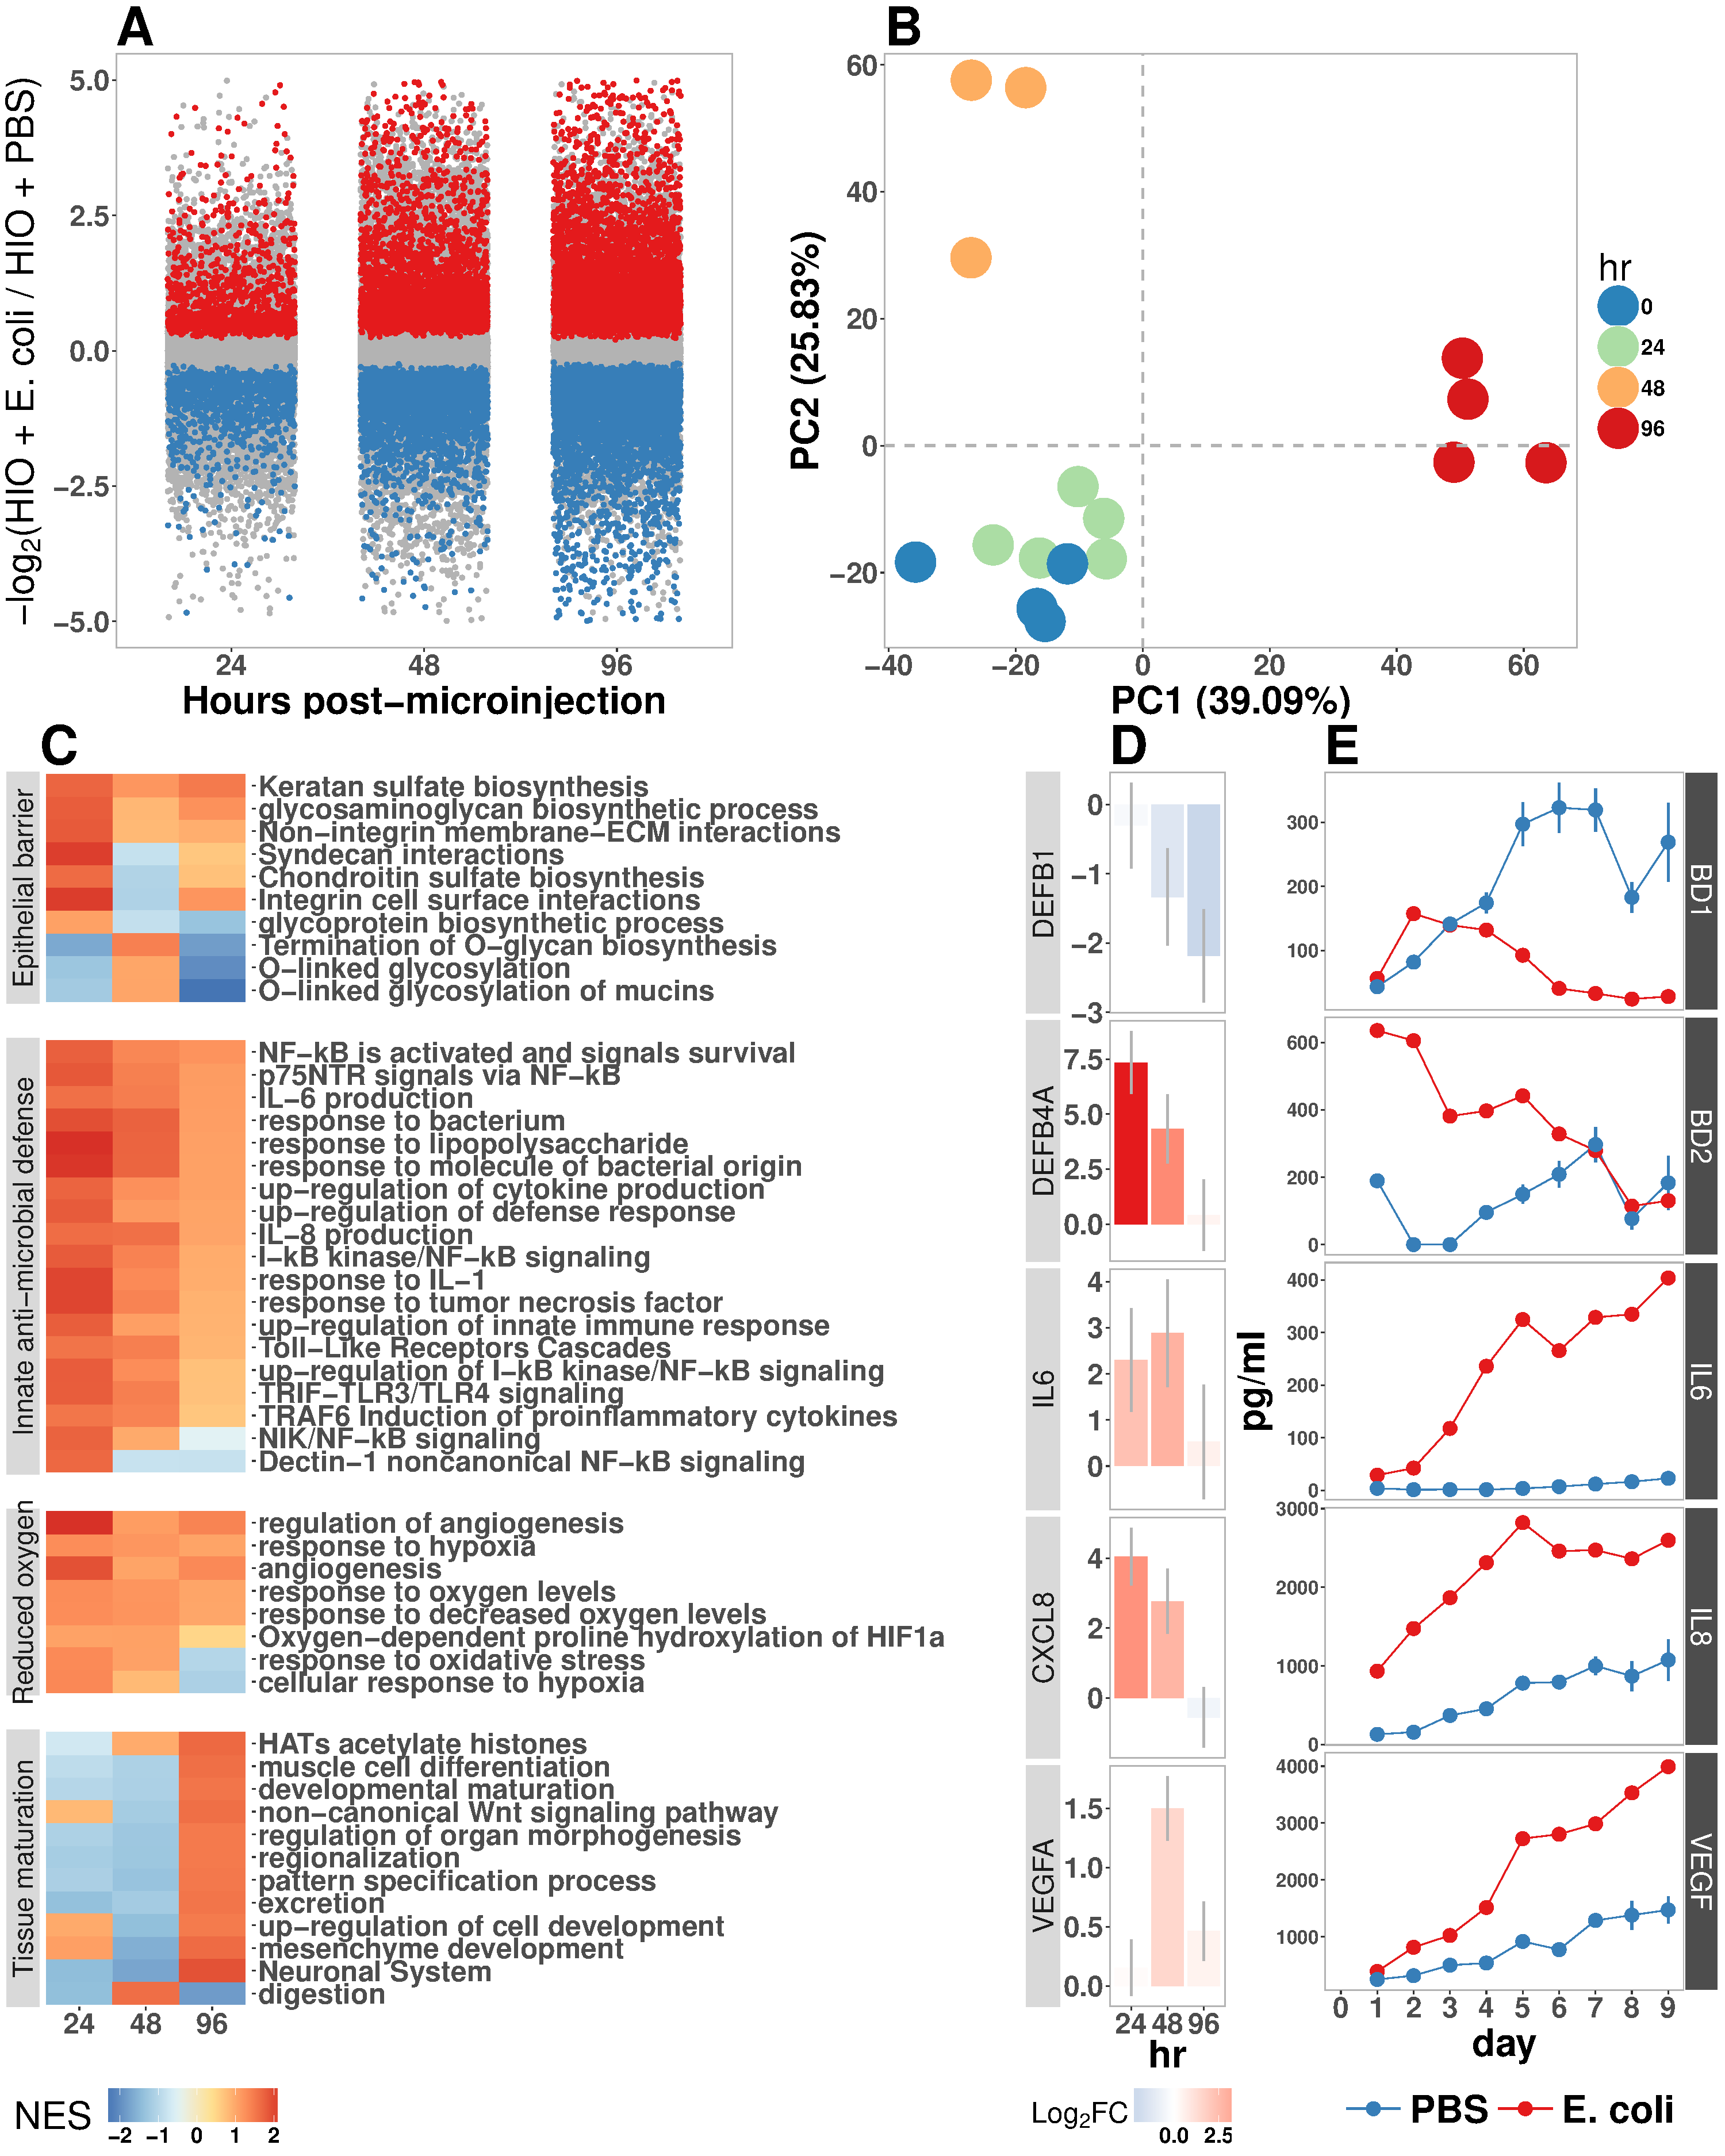
\includegraphics[width=0.85\linewidth]{./figures/figure2/figure2_multipanel.pdf}
\caption{\textbf{A} Log2-transformed fold change in normalized RNA-seq gene counts in \textit{E. coli} associated HIOs at 24, 48, and 96 h post-microinjection relative to PBS-injected HIOs. Differentially expressed genes (adjusted FDR < 0.05) are indicated in red (up-regulated) or blue (down-regulated). \textbf{B} Principle component plot of HIOs at 0-96 h post-microinjection derrived from whole-transcriptome RNA-seq normalized gene counts. Cumulative explained variance for PC1 and PC2 is indicated as a percentage on the x- and y-axes, respectively. \textbf{C} Heat map of normalized enrichment scores (NES) from GSEA of normalized RNA-seq expression data using the GO and REACTOME databases. A positive value of NES indicates activation of a given gene set and a negative value suggests relative suppression of a gene set. All NES scores are calculated relative to PBS-microinjected controls. \textbf{D} Mean log$_{2}$ fold change in normalized RNA-seq gene counts at 24-96 h post microinjection relative to PBS-injected control HIOs. \textbf{E} Protein secretion at 0-9 days post-microinjection with PBS or \textit{E. coli} as measured by ELISA in the supernatant of HIO cultures. The genes given in D correspond to the proteins measured in E.}
\label{fig:fullwidth}
\end{fullwidth}
\end{figure}

\subsection*{{\bfseries\sffamily } \emph{E. coli} colonization is associated with a reduction in luminal O\(_{\text{2}}\)}
\label{sec:orgheadline5}
The mature intestinal epithelium is characterized by a steep oxygen gradient, ranging from 8\% oxygen within the bowel wall to < 2\% oxygen in the lumen of the small intestine \citep{Fisher:2013}. Reduction of oxygen content in the intestinal lumen occurs during the immediate perinatal period \citep{Gruette:1965}, resulting in changes in epithelial physiology \citep{Glover:2016,Kelly:2015,Colgan:2013,Zeitouni:2016} and shaping the subsequent composition of the microbiota \citep{Schmidt:2014,Espey:2013,Albenberg:2014,Palmer:2007,Koenig:2011}. Analysis of the global transcriptional response to \emph{E. coli} association in the immature intestinal tissue revealed pronounced and coordinated changes in gene expression consistent with the onset of hypoxia (\textbf{Figure 2C-E}). We therefore measured oxygen concentration in the lumen of control HIOs and following microinjection of live \emph{E. coli} using a 50 \(\mu\)m diameter fiberoptic optode (\textbf{Figure 3A-B}). Baseline oxygen concentration in the organoid lumen was 8.04 \textpm{} 0.48\%, which was significantly reduced relative to the external culture media (18.86 \textpm{} 0.37\%, \emph{P} = \num{3.6e-11}). At 24 and 48 h post-microinjection, luminal oxygen concentration was significantly reduced in \emph{E. coli}-injected HIOs relative to PBS-injected HIOs (\emph{P} = \num{0.04} and \emph{P} = \num{5.2e-05}, respectively) reaching concentrations as low as 1.67 \textpm{} 0.62\% at 48 h (\textbf{Figure 3A}). \emph{E. coli} injected HIOs were collected and CFU were enumerated from luminal contents at 24 and 48 h post-microinjection. We observed a highly significant negative correlation between luminal CFU and luminal oxygen concentration where increased density of luminal bacteria was correlated with lower oxygen concentrations (r\(^{\text{2}}\) = 0.842, \emph{P} = \num{6.86e-05}; \textbf{Figure 3B}). Finally, in order to assess relative oxygenation in the epithelium itself, we utilized a small molecule pimonidazole (PMDZ), which forms covalent conjugates with thiol groups on cytoplasmic proteins only under low-oxygen conditions \citep{Arteel:1998}. Fluorescent immunohistology demonstrated enhanced PMDZ uptake in \emph{E. coli} associated HIO epithelium relative to PBS-injected HIOs at 48 h post-microinjection (\textbf{Figure 3C}). PMDZ staining was limited to the epithelium and was not detected in the underlying mesenchymal tissue. Thus, luminal and epithelial oxygen concentration is reduced following microinjection of \emph{E. coli} into the HIO, consistent with data in mice showing that the in \emph{vivo} epithelium is in a similar low-oxygen state in normal physiological conditions \citep{Schmidt:2014,Kelly:2015,Kim:2017}.

\begin{figure}
\begin{fullwidth}
\centering
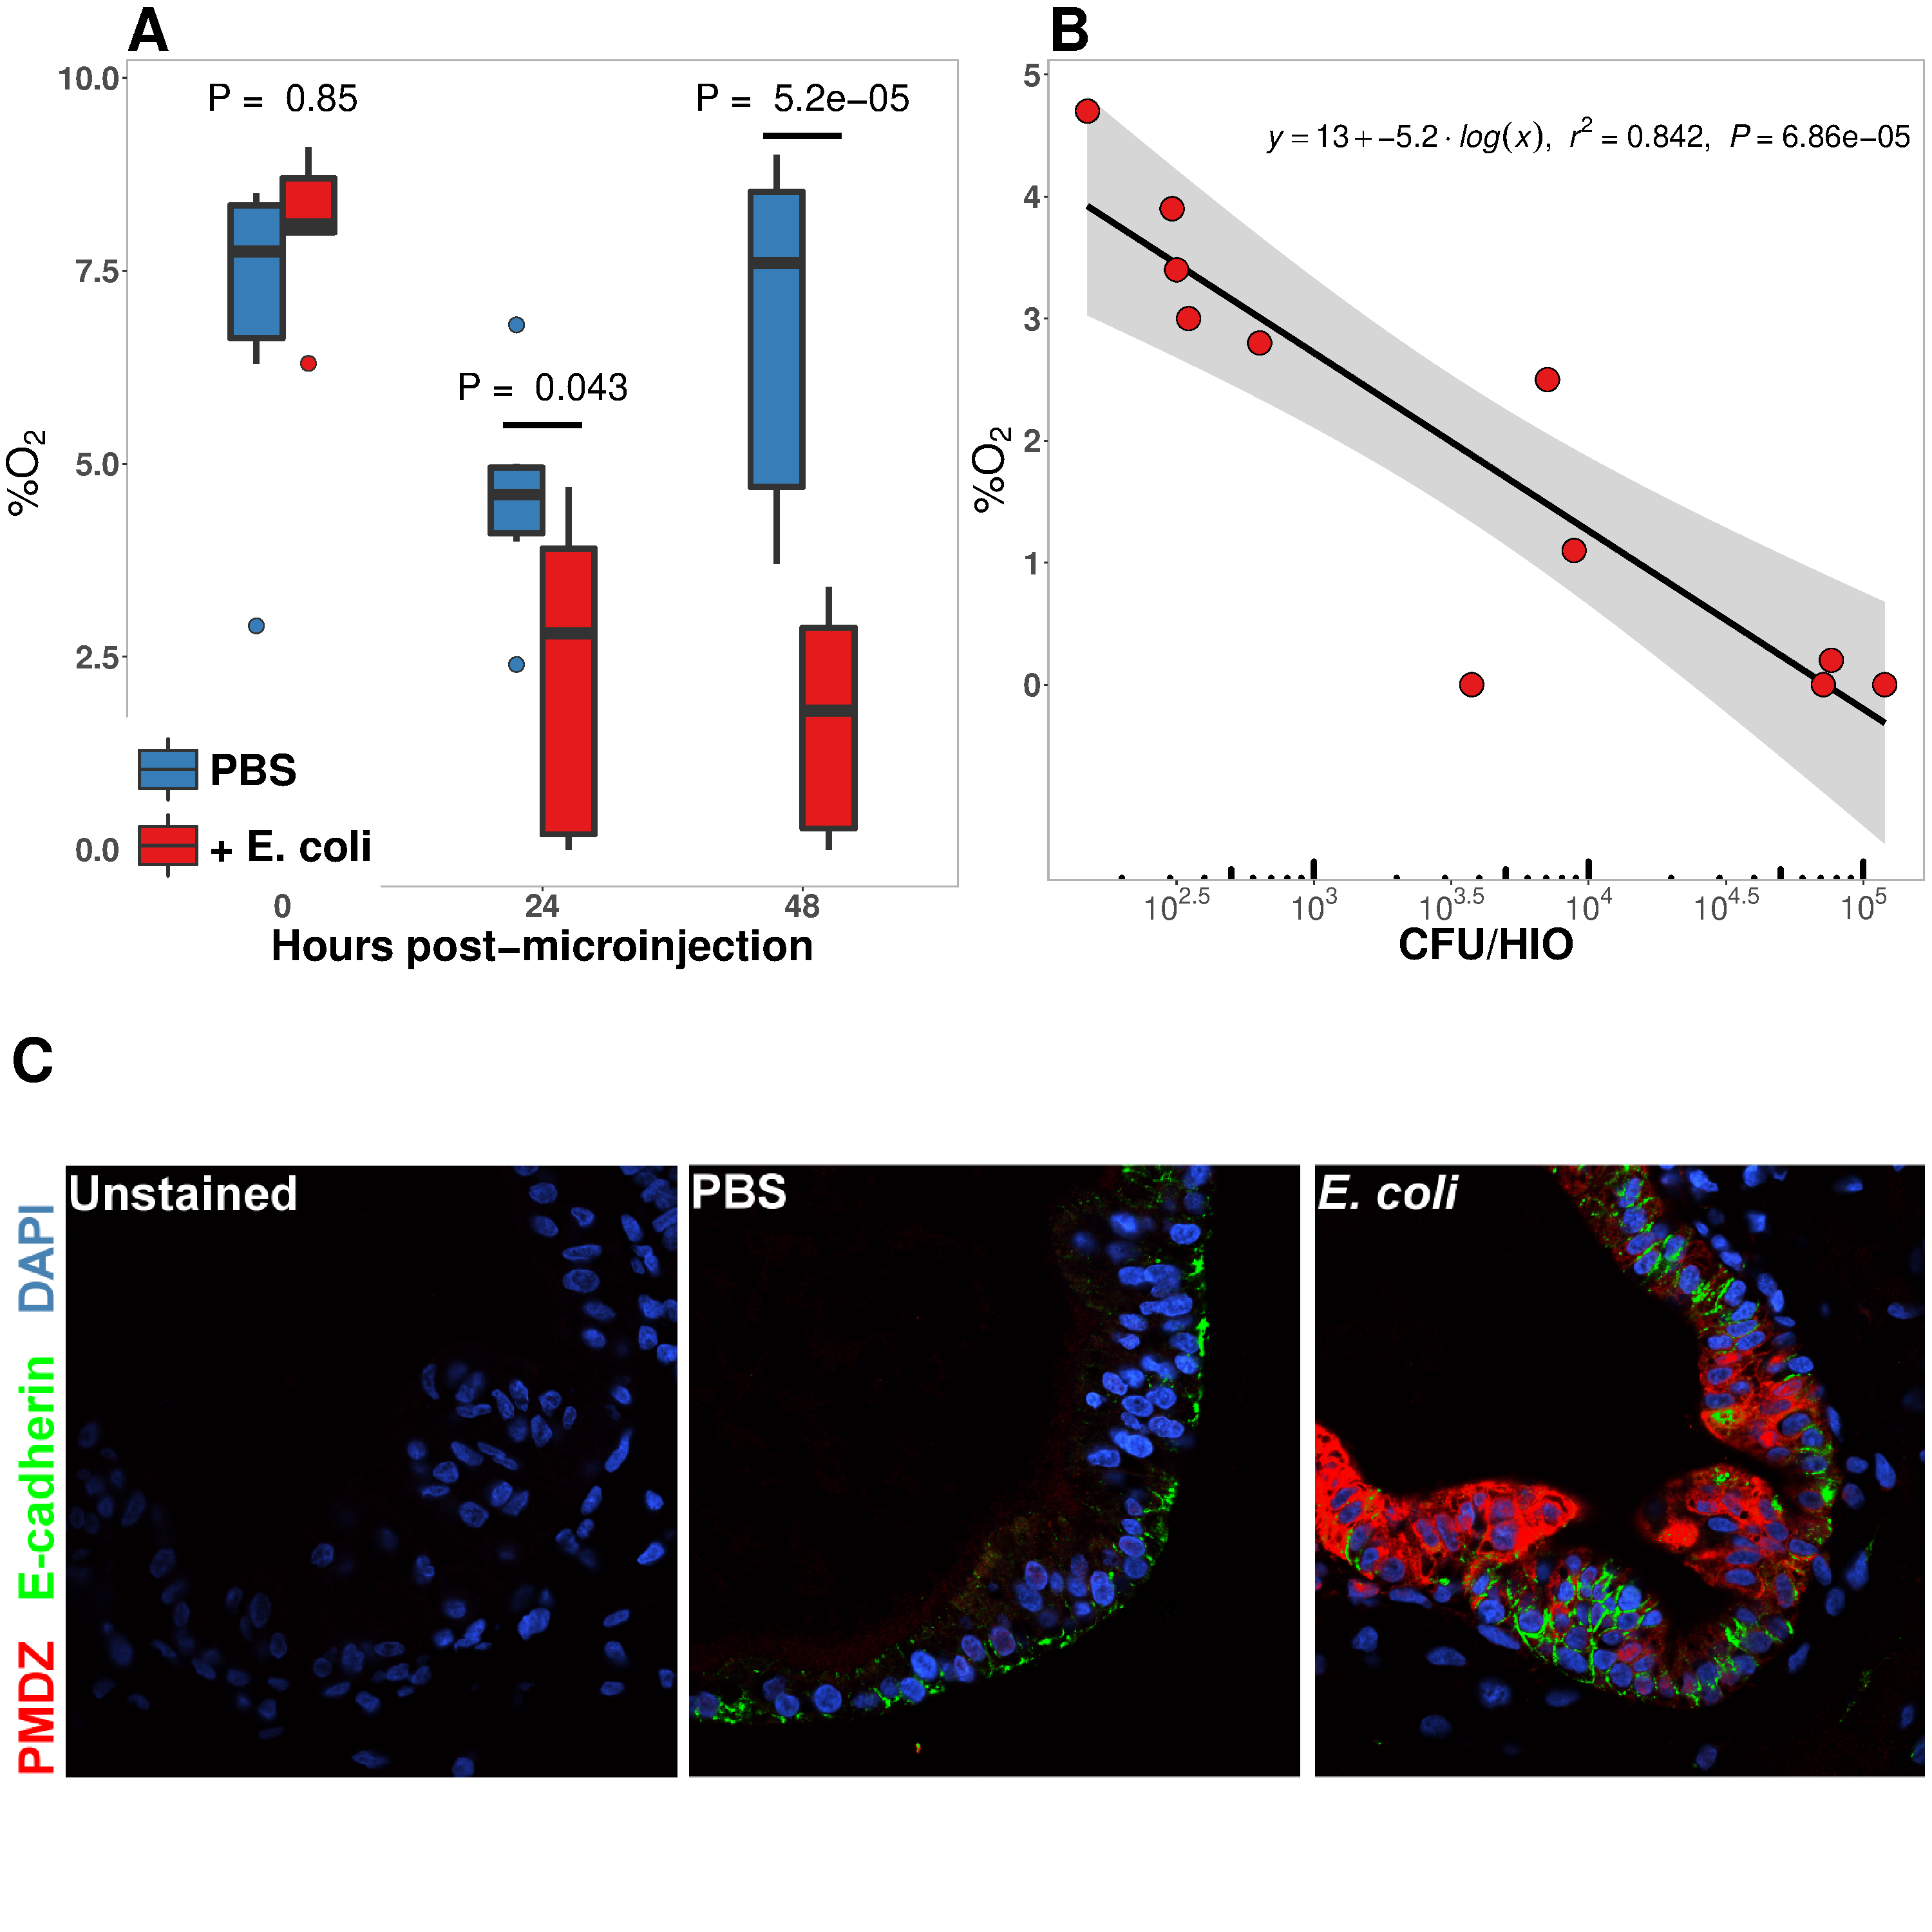
\includegraphics[width=0.95\textwidth]{./figures/figure3/figure3_multipanel.pdf}
\caption{\textbf{A} Luminal oxygen concentration in human intestinal organoids at 0-48 h post-microinjection. \textit{P} values reflect results of unpaired one-tailed Students \textit{t}-tests for the comparisons indicated. \textbf{B} Linear regression analysis of luminal CFU \textit{E. coli} per organoid and luminal oxygen concentration in the same organoid. \textbf{C} Confocal micrographs of the HIO epithelium in PBS- and \textit{E. coli}-injected HIOs at 48 h post-microinjection. The panel marked 'unstained' shows a section in which no primary antibody was applied.}
\label{fig:fullwidth}
\end{fullwidth}
\end{figure}

\subsection*{{\bfseries\sffamily } NF-\(\kappa\)B integrates complex microbial and hypoxic stimuli}
\label{sec:orgheadline6}
\emph{E. coli} association elicits a robust transcriptional response in immature intestinal tissue (\textbf{Figure 2}) that is associated with the onset of luminal oxygen depletion and relative tissue hypoxia (\textbf{Figure 3}). We set out to determine whether we could assign discrete portions of the transcriptional response to direct interaction with microbes or to the subsequent depletion of luminal oxygen. In the RNA-seq analysis (\textbf{Figure 2}), NF-\(\kappa\)B signaling emerged as a major pathway involved in this complex host-microbe interaction, and NF-\(\kappa\)B has been shown by others to act as a transcriptional mediator of both microbial contact and the response to tissue hypoxia  \citep{Rius:2008,Gilmore:2006,Wullaert:2011}. Gene Ontology and REACTOME pathway analysis showed that NF-\(\kappa\)B signaling components are also highly up-regulated following microinjection of \emph{E. coli} into HIOs (\textbf{Figure 2C} and \textbf{Figure 4 - Supplement 1}).  Thus we assessed the role of NF-\(\kappa\)B signaling in the microbial contact-associated transcriptional response and the hypoxia-associated response using the highly selective IKK\(\beta\) inhibitor SC-514 \citep{Kishore:2003,Litvak:2009} to inhibit phosphorylation and activation of the transcription factor p65 (\textbf{Figure 4 - Supplement 2}). Another set of HIOs was simultaneously transferred to a hypoxic chamber and cultured in 1\% O\(_{\text{2}}\) with and without SC-514. At 24 h post-treatment, HIOs were harvested for RNA isolation and RNA-seq. We devised an experimental scheme that allowed us to parse out the relative contributions of microbial contact and microbe-associated luminal hypoxia in the transcriptional response to association with live \emph{E. coli} (\textbf{Figure 4A}). First, we identified a set of genes significantly up-regulated (adjusted FDR < 0.05) by microinjection of either live \emph{E. coli} or heat-inactivated \emph{E. coli} (contact dependent genes). From this gene set, we identified a subset that was suppressed by the presence of NF-\(\kappa\)B inhibitor SC-514 during association with either live or heat-inactivated \emph{E. coli} (Gene Set I, \textbf{Figure 4B}). Thus, Gene Set I represents the NF-\(\kappa\)B dependent transcriptional response to live or dead \emph{E. coli}. Genes induced by live or heat-inactivated \emph{E. coli} but not suppressed by SC-514 were considered NF-\(\kappa\)B independent (Gene Set III, \textbf{Figure 4B}). Likewise, we compared genes commonly up-regulated by association with live \emph{E. coli} and those up-regulated under 1\% O\(_{\text{2}}\) culture conditions. A subset of genes induced by either live \emph{E. coli} or 1\% O\(_{\text{2}}\) culture but suppressed by the presence of NF-\(\kappa\)B inhibitor was identified as the NF-\(\kappa\)B-dependent hypoxia-associated transcriptional response (Gene Set II, \textbf{Figure 4B}). Genes induced by live \emph{E. coli} or hypoxia but not inhibited by the presence of NF-\(\kappa\)B inhibitor were considered NF-\(\kappa\)B independent transcriptional responses to microbe-associated hypoxia (Gene Set IV). Gene lists for each gene set are found in \textbf{Supplementary  File 2}.

Following the identification of these 4 gene sets, we then applied over-representation analysis using the GO and REACTOME pathway databases to identify enriched pathways for each of the 4 gene sets, resulting in 4 clearly distinguishable patterns of gene pathway enrichment (\textbf{Figure 4C}). Contact with either live or heat-inactivated \emph{E. coli} is sufficient to promote expression of genes involved in maintaining epithelial barrier integrity and mucin production, an effect that is suppressed in the presence of NF-\(\kappa\)B inhibitor. Additionally, key developmental pathways including epithelial morphogenesis, digestive tract development, and expression of digestive enzymes appear to be driven primarily by bacterial association and are largely NF-\(\kappa\)B dependent. Robust innate and adaptive defense requires both bacterial contact and hypoxia, with some genes associated with antigen processing and cytokine signaling being NF-\(\kappa\)B dependent (Gene Set II) and others associated with NF-\(\kappa\)B independent gene sets (Gene Sets III \& IV). Genes associated with antimicrobial defensin peptides were enriched only in the hypoxia asociated, NF-\(\kappa\)B independent gene set (Gene Set IV), suggesting that antimicrobial peptides are regulated by mechanisms that are distinct from other aspects of epithelial barrier integrity such as mucins and epithelial junctions (Gene Set I). TLR signaling components were is broadly enhanced by live \emph{E. coli} and associated with both microbial contact and hypoxia were largely NF-\(\kappa\)B independent (Gene Sets III \& IV). Finally, there was a notable transcriptional signature suggesting metabolic and mitochondrial adaptation to bacteria that was independent of NF-\(\kappa\)B and primarily driven by bacterial contact rather than hypoxia (Gene Set III). Taken together, this analysis demonstrates that association of immature intestinal epithelium with live \emph{E. coli} results in a complex interplay between microbial contact and microbe-associated hypoxia induced gene expression. 

\begin{figure}
\begin{fullwidth}
\centering
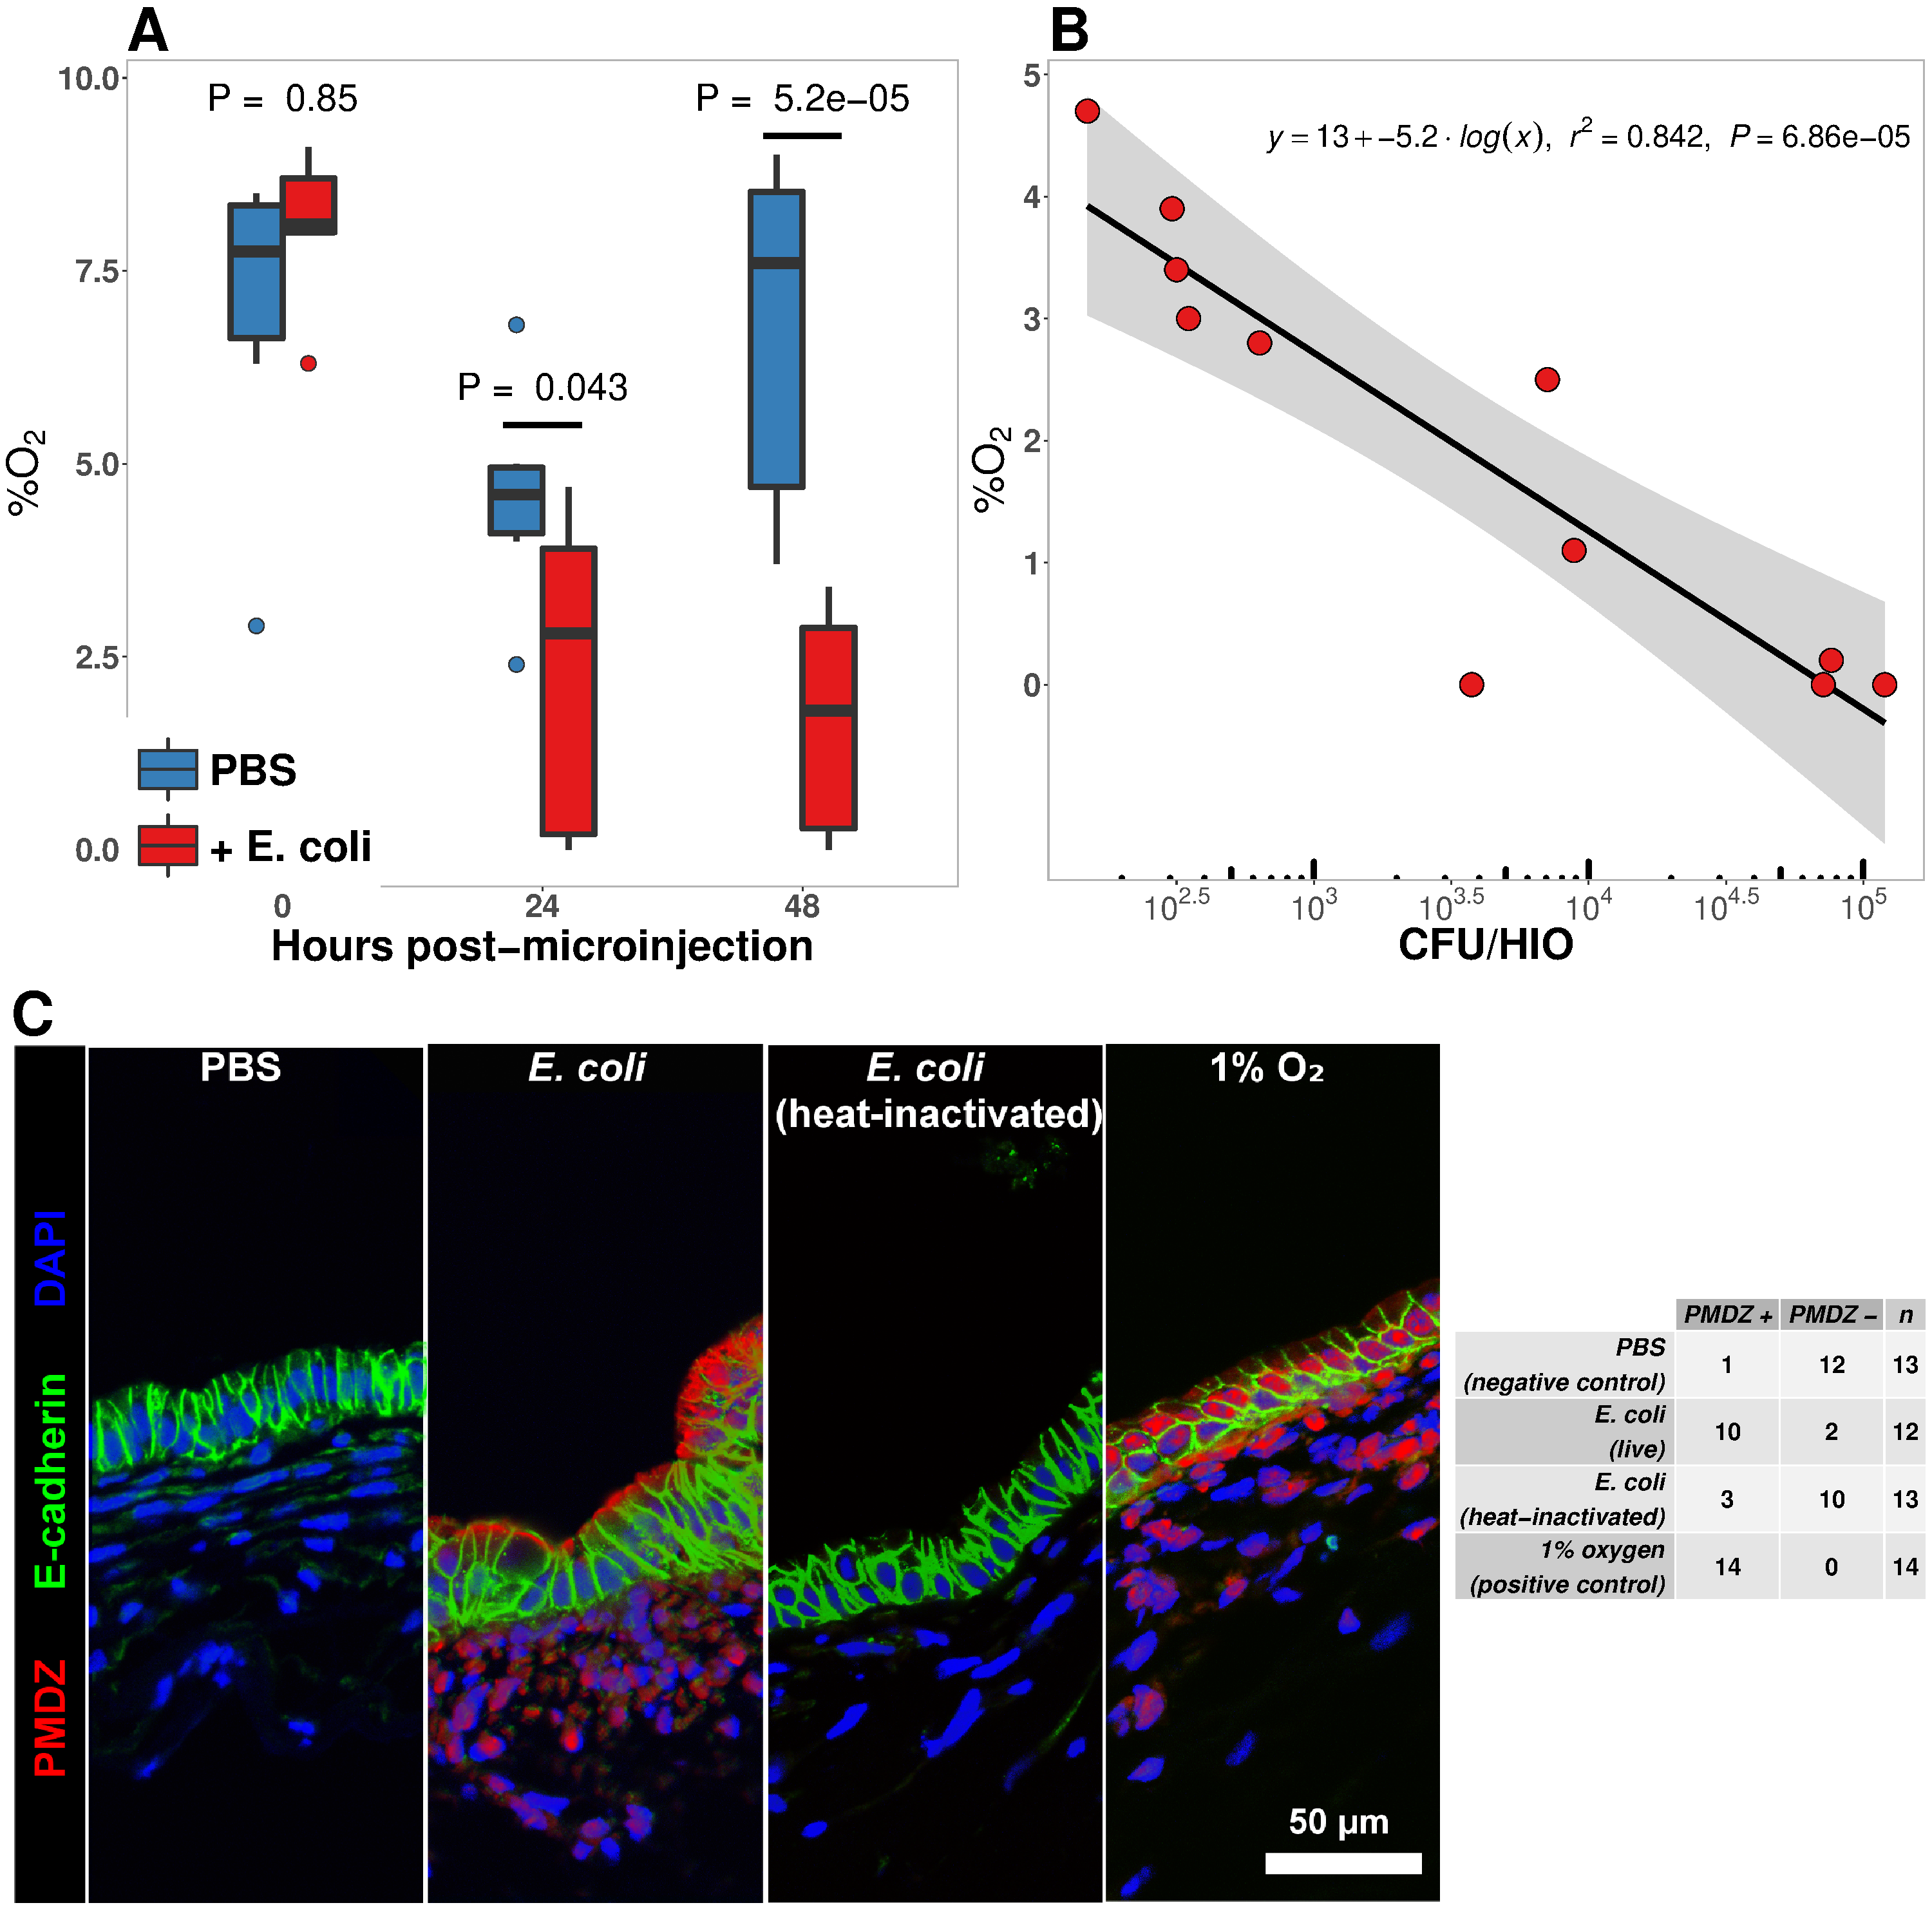
\includegraphics[width=0.95\textwidth]{./figures/figure4/figure4_multipanel.pdf}
\caption{\textbf{A} Analysis scheme for identifying genes sets representing the components of the transcriptional response to live \textit{E. coli} that could be recapitulated with heat-inactivated \textit{E. coli} (contact induced) or hypoxia (microbial-associated hypoxia induced) as well as the subsets of genes induced through NF-$\kappa$B dependent signaling. \textbf{B} Scatter plots with density overlay indicating the genes meeting the \textit{a priori} criteria identified in panel A. \textbf{C} Bar plot of the proportion of genes in the input gene sets mapping to each pathway from the GO and REACTOME databases enrichment \textit{P}-values for each of the gene sets identified in A. Pathways with enrichment \textit{P}-values < 0.01 were excluded from the plot.}
\label{fig:fullwidth}
\end{fullwidth}
\end{figure}

\subsection*{{\bfseries\sffamily } Bacterial association promotes secretion of antimicrobial peptides}
\label{sec:orgheadline7}
Antimicrobial peptides (AMPs) are key effectors for innate defense of epithelial surfaces \citep{Muniz:2012} and act to inhibit microbial growth through direct lysis of the bacterial cell wall and modulation of bacterial metabolism  \citep{Ganz:2003,Bevins:2011,O'Neil:2003,Vora:2004,Brogden:2005}. Defensin gene expression is highly up-regulated following microinjection of \emph{E. coli} into HIOs (\textbf{Figures 2D-E and 4C}). Using an annotated database of known AMPs \citep{Wang:2016} to query our RNA-seq datasets, we found that several AMPs are up-regulated in the immature intestinal epithelium following \emph{E. coli} association (\textbf{Figure 5A}). Among these, DEFB4A and DEFB4B, duplicate genes encoding the peptide human \(\beta\)-defensin 2, were the most highly up-regulated; other AMPs induced by \emph{E. coli} association included multi-functional peptides CCL20, CXCL2, CXCL1, CXCL6, CXCL3, REG3A \citep{Cash:2006}, and LTF (\textbf{Figure 5A}). Analysis of RNA-seq data from HIOs microinjected with live or heat-killed \emph{E .coli} with and without NF-\(\kappa\)B inhibitor or culture of HIOs under hypoxic conditions had indicated that defensin genes were enriched among the set of NF-\(\kappa\)B-independent genes induced by hypoxia (\textbf{Figure 4C}). We examined \emph{DEFB4A} expression specifically (\textbf{Figure 5B}) and found that relative to control treatment, microinjection of live \emph{E. coli} resulted in a 7.38-fold increase in normalized \emph{DEFB4A} expression. Consistent with the notion that \emph{DEFB4A} expression is induced by hypoxia and is not dependent on NF-\(\kappa\)B signaling, NF-\(\kappa\)B inhibitor treated HIOs injected with E. coli still showed an \textasciitilde{}8-fold increase in gene expression and hypoxia-cultured HIOs showed a \textasciitilde{}5.5 fold induction (\textbf{Figure 5B}). On the other hand, microinjection with heat-inactivated \emph{E. coli} resulted in \emph{DEFB4A} induction that was significantly lower relative to microinjection with live \emph{E. coli} (\emph{P} = 0.007. A similar pattern of expression was observed for \emph{DEFB4B} (\textbf{Figure 5 - Supplement 1}).

We also examined secretion of human \(\beta\)-defensin 2 peptide (BD-2) in the supernatant of \emph{E. coli} associated HIOs (\textbf{Figure 2E} and \textbf{Figure 5C}). BD-2 secretion was increased 3.4-fold at 24 h following \emph{E. coli} microinjection (\emph{P} = \num{2.7e-08}). 
However, heat-inactivation of \emph{E. coli} or addition of NF-\(\kappa\)B inhibitor resulted in suppression of BD-2 secretion relative to live \emph{E. coli} (\emph{P} = \num{0.00051} and \num{1.6e-06}, respectively). To determine if the levels of BD-2 produced by HIOs and secreted into the media were sufficient to retard bacterial growth, we tested the effect of BD-2 at concentrations recapitulating the baseline state in the HIO (\textasciitilde{}0.1 \(\mu\)g/mL) and following microinjection with \emph{E.coli} (\textasciitilde{}1 \(\mu\)g/mL) on \emph{in vitro} growth of \emph{E. coli} over 18 h (\textbf{Figure 5D}). Although there was little effect on \emph{E. coli} density during initial log-phase growth, BD-2 reduced the amount of time bacteria spent in log-phase growth, and \emph{E. coli} density was significantly decreased over time in bacterial growth media supplemented BD-2 (\emph{P} = \num{0.001}). Furthermore, concentrations of BD-2 consistent those found in HIO-/E. coli/ supernatant (1\(\mu\)g/mL) was significantly more inhibitory than low concentration BD-2 (0.1 \(\mu\)g/mL) in our \emph{in vitro} growth assay (\emph{P} = 0.013). From this experiment we conclude that \emph{E. coli} association promotes enhanced expression of AMPs, including BD-2, at concentrations that are sufficient to suppress microbial growth.

\begin{figure}
\begin{fullwidth}
\centering
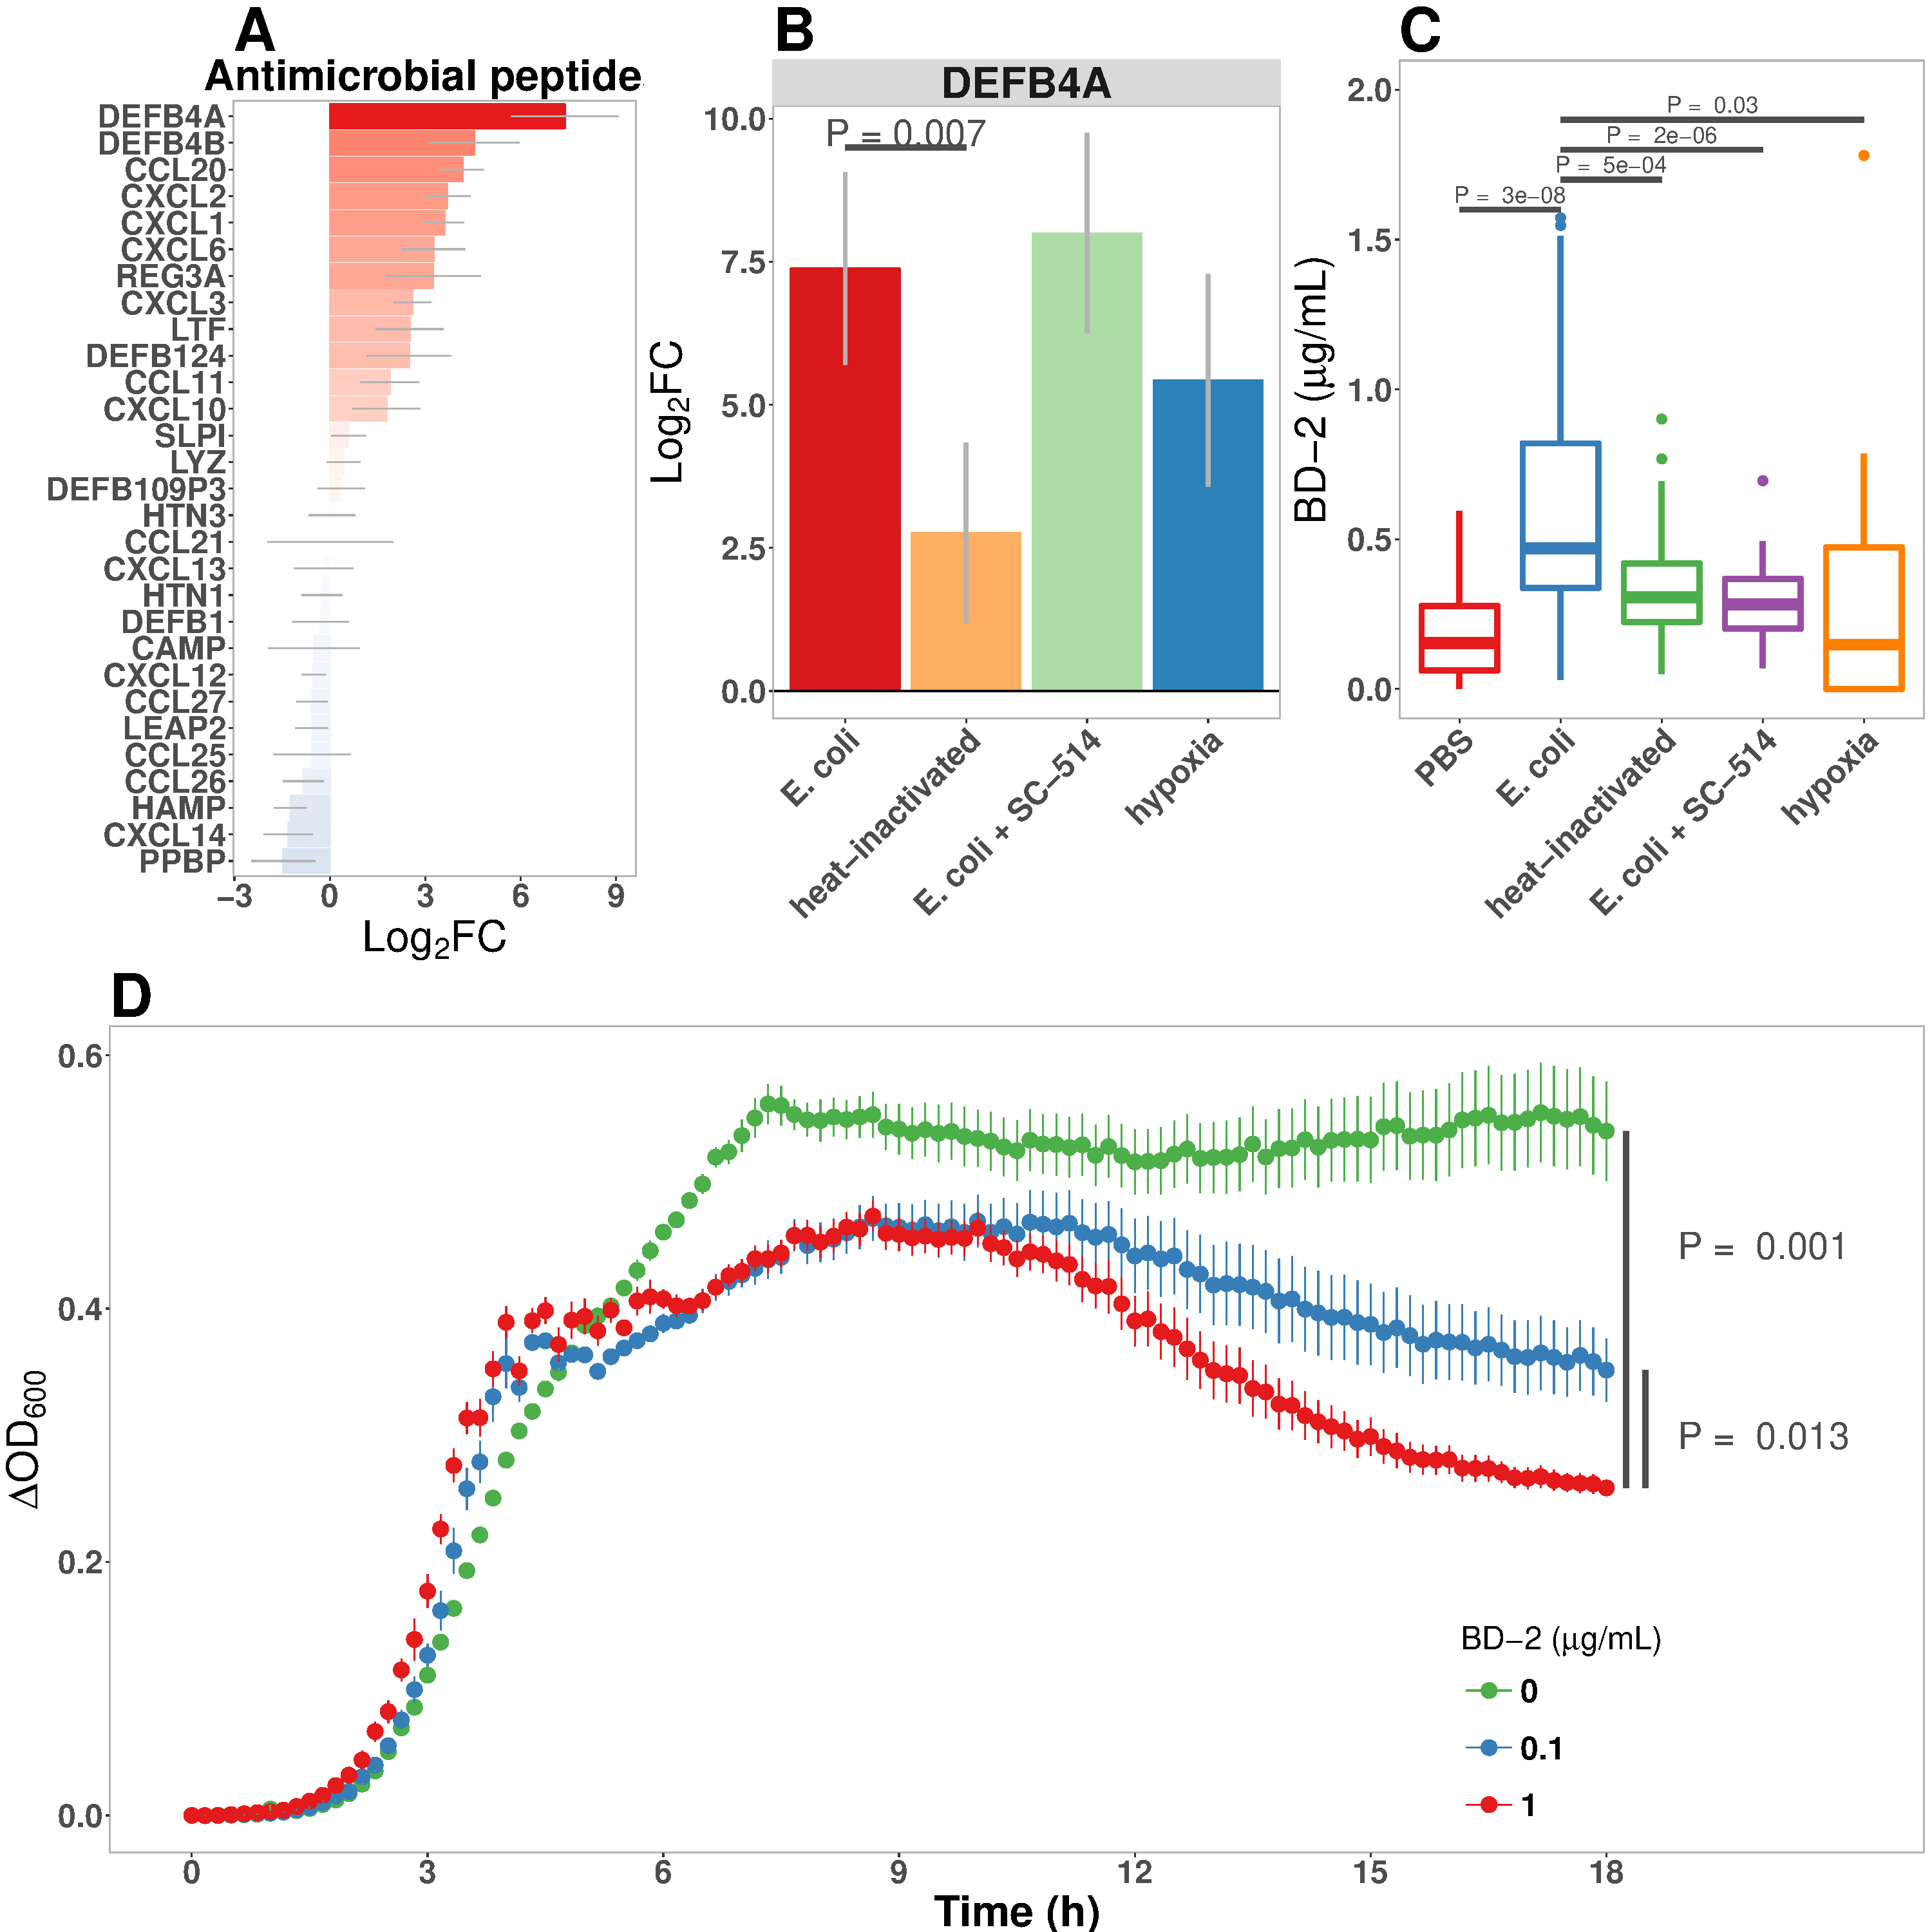
\includegraphics[width=0.95\linewidth]{./figures/figure5/figure5_multipanel.pdf}
\caption{\textbf{A} Normalized fold change in antimicrobial peptide (AMP) gene expression in \textit{E. coli}-associated HIOs at 24 h relative to PBS control treatment. \textbf{B} Normalized fold change in expression of DEFB4A, the gene encoding human $\beta$-defensin 2 (BD-2) peptide, in each of the conditions indicated relative to PBS control treatment. \textbf{C} Concentration of BD-2 peptide in culture supernatant at 24 h as measured by ELISA in HIO cultures treated as indicated. \textbf{D}. Optical density (600 nm) of \textit{E. coli} suspension cultures supplemented with PBS or BD-2 at 10 min intervals over an 18 h period at \SI{37}{\celsius}. \textit{P} values represents the results of a two-tailed Student's \textit{t}-test  for the comparisons indicated.}
\label{fig:fullwidth}
\end{fullwidth}
\end{figure}

\subsection*{{\bfseries\sffamily } Bacterial colonization promotes expression of epithelial mucins and glycotransferases}
\label{sec:orgheadline8}
Mucins are an essential component of epithelial integrity, serving as a formidable barrier to microbial invasion and repository for secreted AMPs \citep{Bergstrom:2013,Cornick:2015,Johansson:2016,Kim:2010}. Mucin synthesis requires a complex series of post-translational modifications that add high molecular weight carbohydrate side chains to the core mucin protein \citep{varki2017essentials}. Our RNA-seq data suggested that mucin gene expression is dependent on both bacterial contact and NF-\(\kappa\)B signaling (\textbf{Figure 4C}). Therefore, we examined expression of genes in control and \emph{E. coli} microinjected HIOs that encode mucin core proteins as well as the glycotransferases that generate the wide variety of post-translational mucin modifications (\textbf{Figure 6A}). Although some glycotransferases were increased at 24 h after \emph{E. coli} microinjection, expression of mucin core proteins and many glycotransferases reached peak levels at 48 h after the introduction of \emph{E. coli} to the HIO lumen (\textbf{Figure 6A}). Periodic Acid-Schiff and Alcian blue staining (PAS/AB) of sections taken from HIOs at 48 h after \emph{E. coli} microinjection reveal the formation of a robust mucin layer at the apical epithelial surface consisting of both acidic (AB-positive) and neutral (PAS-positive) glycoprotein components, suggesting a rich matrix of O-linked mucins, glycosaminoglycans, and proteoglycans (\textbf{Figures 6B-C}). Interestingly, we observed that \emph{E. coli} association caused an initial induction of \emph{MUC5AC} at 48h that was reduced by 96 h (\textbf{Figure 6A}). \emph{MUC5AC} is most highly expressed within the gastric mucosa, but has also been reported in the duodenal epithelium \citep{Buisine:1998,Buisine:2001,Rodriguez-Pineiro:2013}. On the other hand, \emph{MUC2} is more commonly associated with the duodenum, and increased more slowly, showing peak expression after 96 hours of association with \emph{E. coli} (\textbf{Figure 6A}). Co-staining of control HIOs and \emph{E. coli} microinjected HIOs demonstrated colocalization with \emph{Ulex europaeus} agglutinin I (UEA1), a lectin with high specificity for the terminal fucose moiety Fuc\(\alpha\)1-2Gal-R (\textbf{Figure 6D}). This suggests that following \emph{E. coli} association, HIOs produce mucins with mature carbohydrate modifications.

RNA-seq data suggested that O-linked mucins were highly enriched among the subset of genes induced by bacterial contact in an NF-\(\kappa\)B-dependent manner (\textbf{Figure 4}). We examined this phenomenon at the level of individual glycosyltransferase and mucin genes (\textbf{Figure 6E}). \emph{E. coli} induced transcription of mucins and glycosyltransferases (\textbf{Figure 6E}) and mucin secretion (\textbf{Figure 6 - Supplement 1})  was suppressed in the presence of NF-\(\kappa\)B inhibitor SC-514. Furthermore, culture of HIOs under hypoxia conditions was not sufficient to promote transcription of genes involved in mucin synthesis (\textbf{Figure 6E}). This result was confirmed with PAS/AB staining of HIOs microinjected with PBS, live or heat-inactivated \emph{E. coli}, or cultured under hypoxic conditions for 24 h, where bacterial contact promoted formation of a mucus layer while PBS microinjection or culture under hypoxic conditions did not (\textbf{Figure 6F}). Taken together, these results indicate that association of the immature intestinal epithelium with \emph{E. coli} promotes robust mucus secretion through an NF-\(\kappa\)B-dependent mechanism and that hypoxia alone is not sufficient to recapitulate \emph{E. coli} induced mucus production.

\begin{figure}
\begin{fullwidth}
\centering
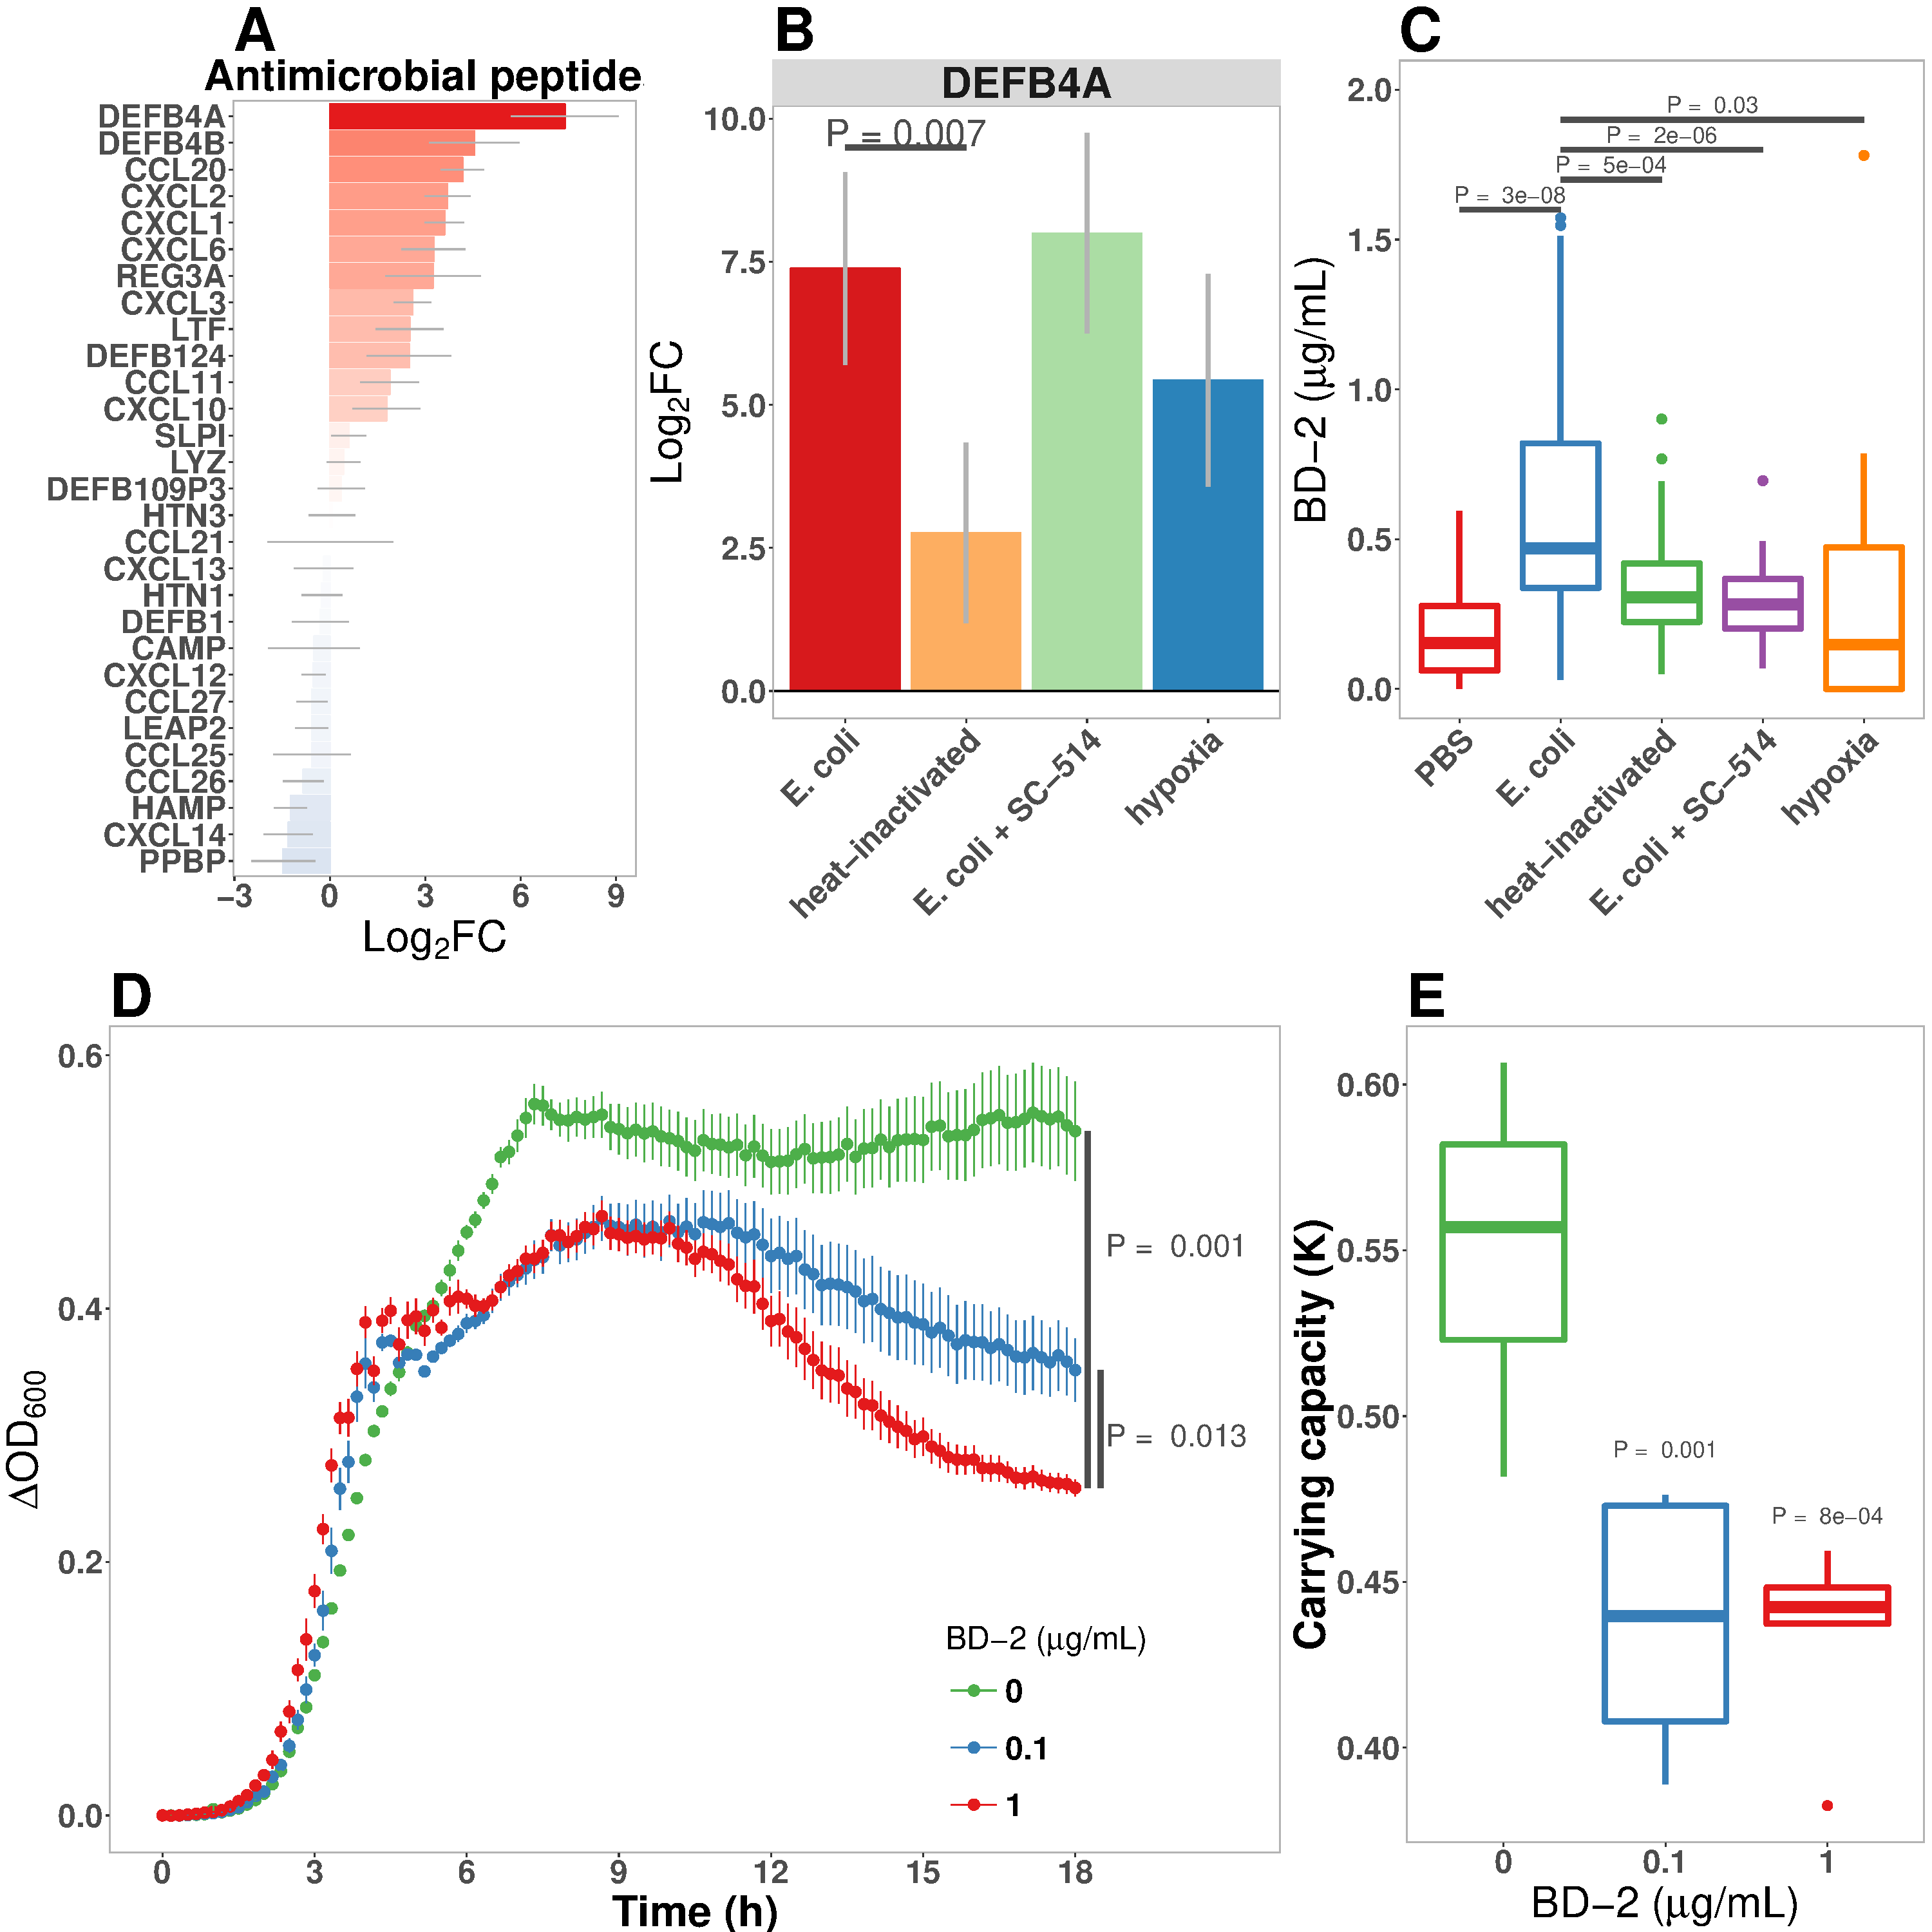
\includegraphics[width=0.9\linewidth]{./figures/figure6/figure6_multipanel.pdf}
\caption{\textbf{A} Heatmap of normalized RNA-seq glycotransferase and mucin gene counts of HIOs associated with \textit{E. coli} at 0-96 h post-microinjection. \textbf{B} Periodic acid-Schiff and Alcian Blue (PAS-AB) staining of control HIOs or HIOs microinjected with \textit{E. coli} and cultured for 48 h at 10X magnification. \textbf{C} HIO epithelium from control HIOs or HIOs microinjected with \textit{E. coli} and cultured for 48 h stained with H\&E, AB, PAS, or PAS-AB and imaged under 100X light microscopy. \textbf{D} Confocal micrograph of HIO epithelium from a control HIO or an HIO microinjected with \textit{E. coli} and cultured for 48 h. Nuclei are stained blue with DAPI, and fluorescent antibody-labeled proteins E-cadherein and Mucin 5 AC are pseudocolored in white or red, respectively. UEA1 lectin is used to label the carbohydrate moiety Fuc$\alpha$1-2Gal-R, which is pseudo colored in green. 60X optical magnification. \textbf{E} Heatmap of normalized RNA-seq glycotransferase and mucin gene counts of HIOs associated with live or heat-inactivated \textit{E. coli}, \textit{E. coli} + NF-$\kappa$B inhibitor (SC-514) or HIOs cultured under hypoxic conditions for 24 h. \textbf{F} PAS-AB staining of HIOs treated as indicated in the figure labels for 24 h. 10X magnification.}
\label{fig:fullwidth}
\end{fullwidth}
\end{figure}
\subsection*{{\bfseries\sffamily } Epithelial barrier integrity is enhanced following bacterial association}
\label{sec:orgheadline9}
Having established that stem-cell derived immature intestinal epithelium (\textbf{Figure 1 - Supplement 1}) can be stably associated with commensal \emph{E. coli} (\textbf{Figure 1}), resulting in broad changes in transcriptional activity (\textbf{Figure 2}) and leading to elevated production of AMPs (\textbf{Figure 5}) and epithelial mucus secretion (\textbf{Figure 6}), we hypothesized that these changes in gene and protein expression would have functional consequences for the immature epithelial barrier. RNA-seq analysis demonstrated broad up-regulation of transcription in genes involved in the formation of the adherens junction and other cell-cell interactions in HIOs after microinjection with live \emph{E. coli} that was inhibited in the presence of NF-\(\kappa\)B inhibitor SC-514 (\textbf{Figure 7A}). We utilized a modified FITC-dextran permeability assay \citep{Leslie:2015} and real-time imaging of live HIO cultures to measure epithelial barrier function in HIOs microinjected with PBS, live \emph{E. coli}, or live \emph{E. coli} + SC-514 at 24 h after microinjection (\textbf{Figure 7B}). While HIOs pre-conditioned by PBS or \emph{E. coli} microinjection retained 94.1 \textpm{} 0.3\% of the FITC-dextran fluorescence over the 20 h assay period, whereas \emph{E. coli} microinjected HIOs cultured in the presence of SC-514 retained only 45.5 \textpm{} 26.3\% of the fluorescent signal (\emph{P} = 0.02; \textbf{Figure 7B}). We also measured the rate of bacterial translocation across the HIO epithelium, which resulted in contaminated culture media (\textbf{Figure 7C}). HIOs microinjected with \emph{E. coli} and cultured \textpm{} SC-514 were compared to HIOs cultured with vehicle (DMSO controls) and PBS microinjected controls over 7 days in culture. HIOs associated with \emph{E. coli} + SC-514 exhibited a rapid onset of bacterial translocation by day 2-3, with bacterial translocation detected in 96\% of SC-514 treated HIOs by day 7 compared to 23\% of HIOs microinjected with \emph{E. coli} and cultured in the absence of SC-514 (\emph{P} = \num{<2e-16}; \textbf{Figure 7C}). Therefore, inhibition of NF-\(\kappa\)B signaling inhibited epithelial barrier maturation resulting in increased bacterial translocation during \emph{E. coli} association with the immature epithelium.

Finally, we assayed epithelial barrier function under circumstances recapitulating physiologic inflammation. TNF\(\alpha\) and IFN\(\gamma\) are key cytokines mediating innate and adaptive immune cell activity in the gut \citep{Turner:2009} during bacterial infection \citep{Rhee:2005,Emami:2012} and in necrotizing enterocolitis \citep{Tan:1993,Ford:1996,Ford:1997,Halpern:2003,Upperman:2005}. The combination of TNF\(\alpha\) and IFN\(\gamma\) has been previously demonstrated to induce barrier permeability in a dose-dependent manner in Transwell epithelial cultures \citep{Wang:2005,Wang:2006}. Thus, HIOs were microinjected with PBS or live \emph{E. coli} and cultured for 24 h, and were subsequently microinjected with FITC-dextran and treated with PBS or a cocktail of TNF\(\alpha\) and IFN\(\gamma\) added to the external media to expose the basolateral epithelium (\textbf{Figure 7D}). Loss of FITC-dextran fluorescence was observed using live-imaging and indicated that treatment with TNF\(\alpha\) and IFN\(\gamma\) alone resulted in a rapid and sustained decrease in luminal fluorescence relative to  PBS or \emph{E. coli} injected HIOs (\emph{P} = \num{5e-04}, \textbf{Figure 7D}). However, HIOs associated with \emph{E. coli} prior to addition of the TNF\(\alpha\) and IFN\(\gamma\) cocktail retained significantly more fluorescent signal relative to treatment with TNF\(\alpha\) and IFN\(\gamma\) alone (\emph{P} = 0.042, \textbf{Figure 7D}). We examined expression and distribution of the tight junction protein ZO-1, and the basal-lateral protein E-cadherin (ECAD)  in histological sections taken from PBS and \emph{E. coli}-associated HIOs subjected to TNF\(\alpha\) and IFN\(\gamma\) treatment (\textbf{Figure 7E}). Compared to controls, the epithelial layer is highly disorganized in HIOs treated with TNF\(\alpha\) and IFN\(\gamma\), with cytoplasmic ZO-1 staining and disorganized ECAD. By contrast, HIOs associated with \emph{E. coli} prior to TNF\(\alpha\) and IFN\(\gamma\) treatment retain and organized columnar epithelium with robust apical ZO-1 and properly localized ECAD staining (\textbf{Figure 7E}). Similarly, proper localization of additional markers of epithelial barrier integrity occludin (OCLN) and acetylated-tubulin are retained in HIOs associated with \emph{E. coli} during TNF\(\alpha\) and IFN\(\gamma\) treatment relative to HIOs treated with TNF\(\alpha\) and IFN\(\gamma\) alone (\textbf{Figure 7 - Supplement 1}).These results suggest that colonization of the immature epithelium with \emph{E. coli} results in an epithelium that is more robust to challenge by potentially damaging inflammatory cytokines.

\begin{figure}
\begin{fullwidth}
\centering
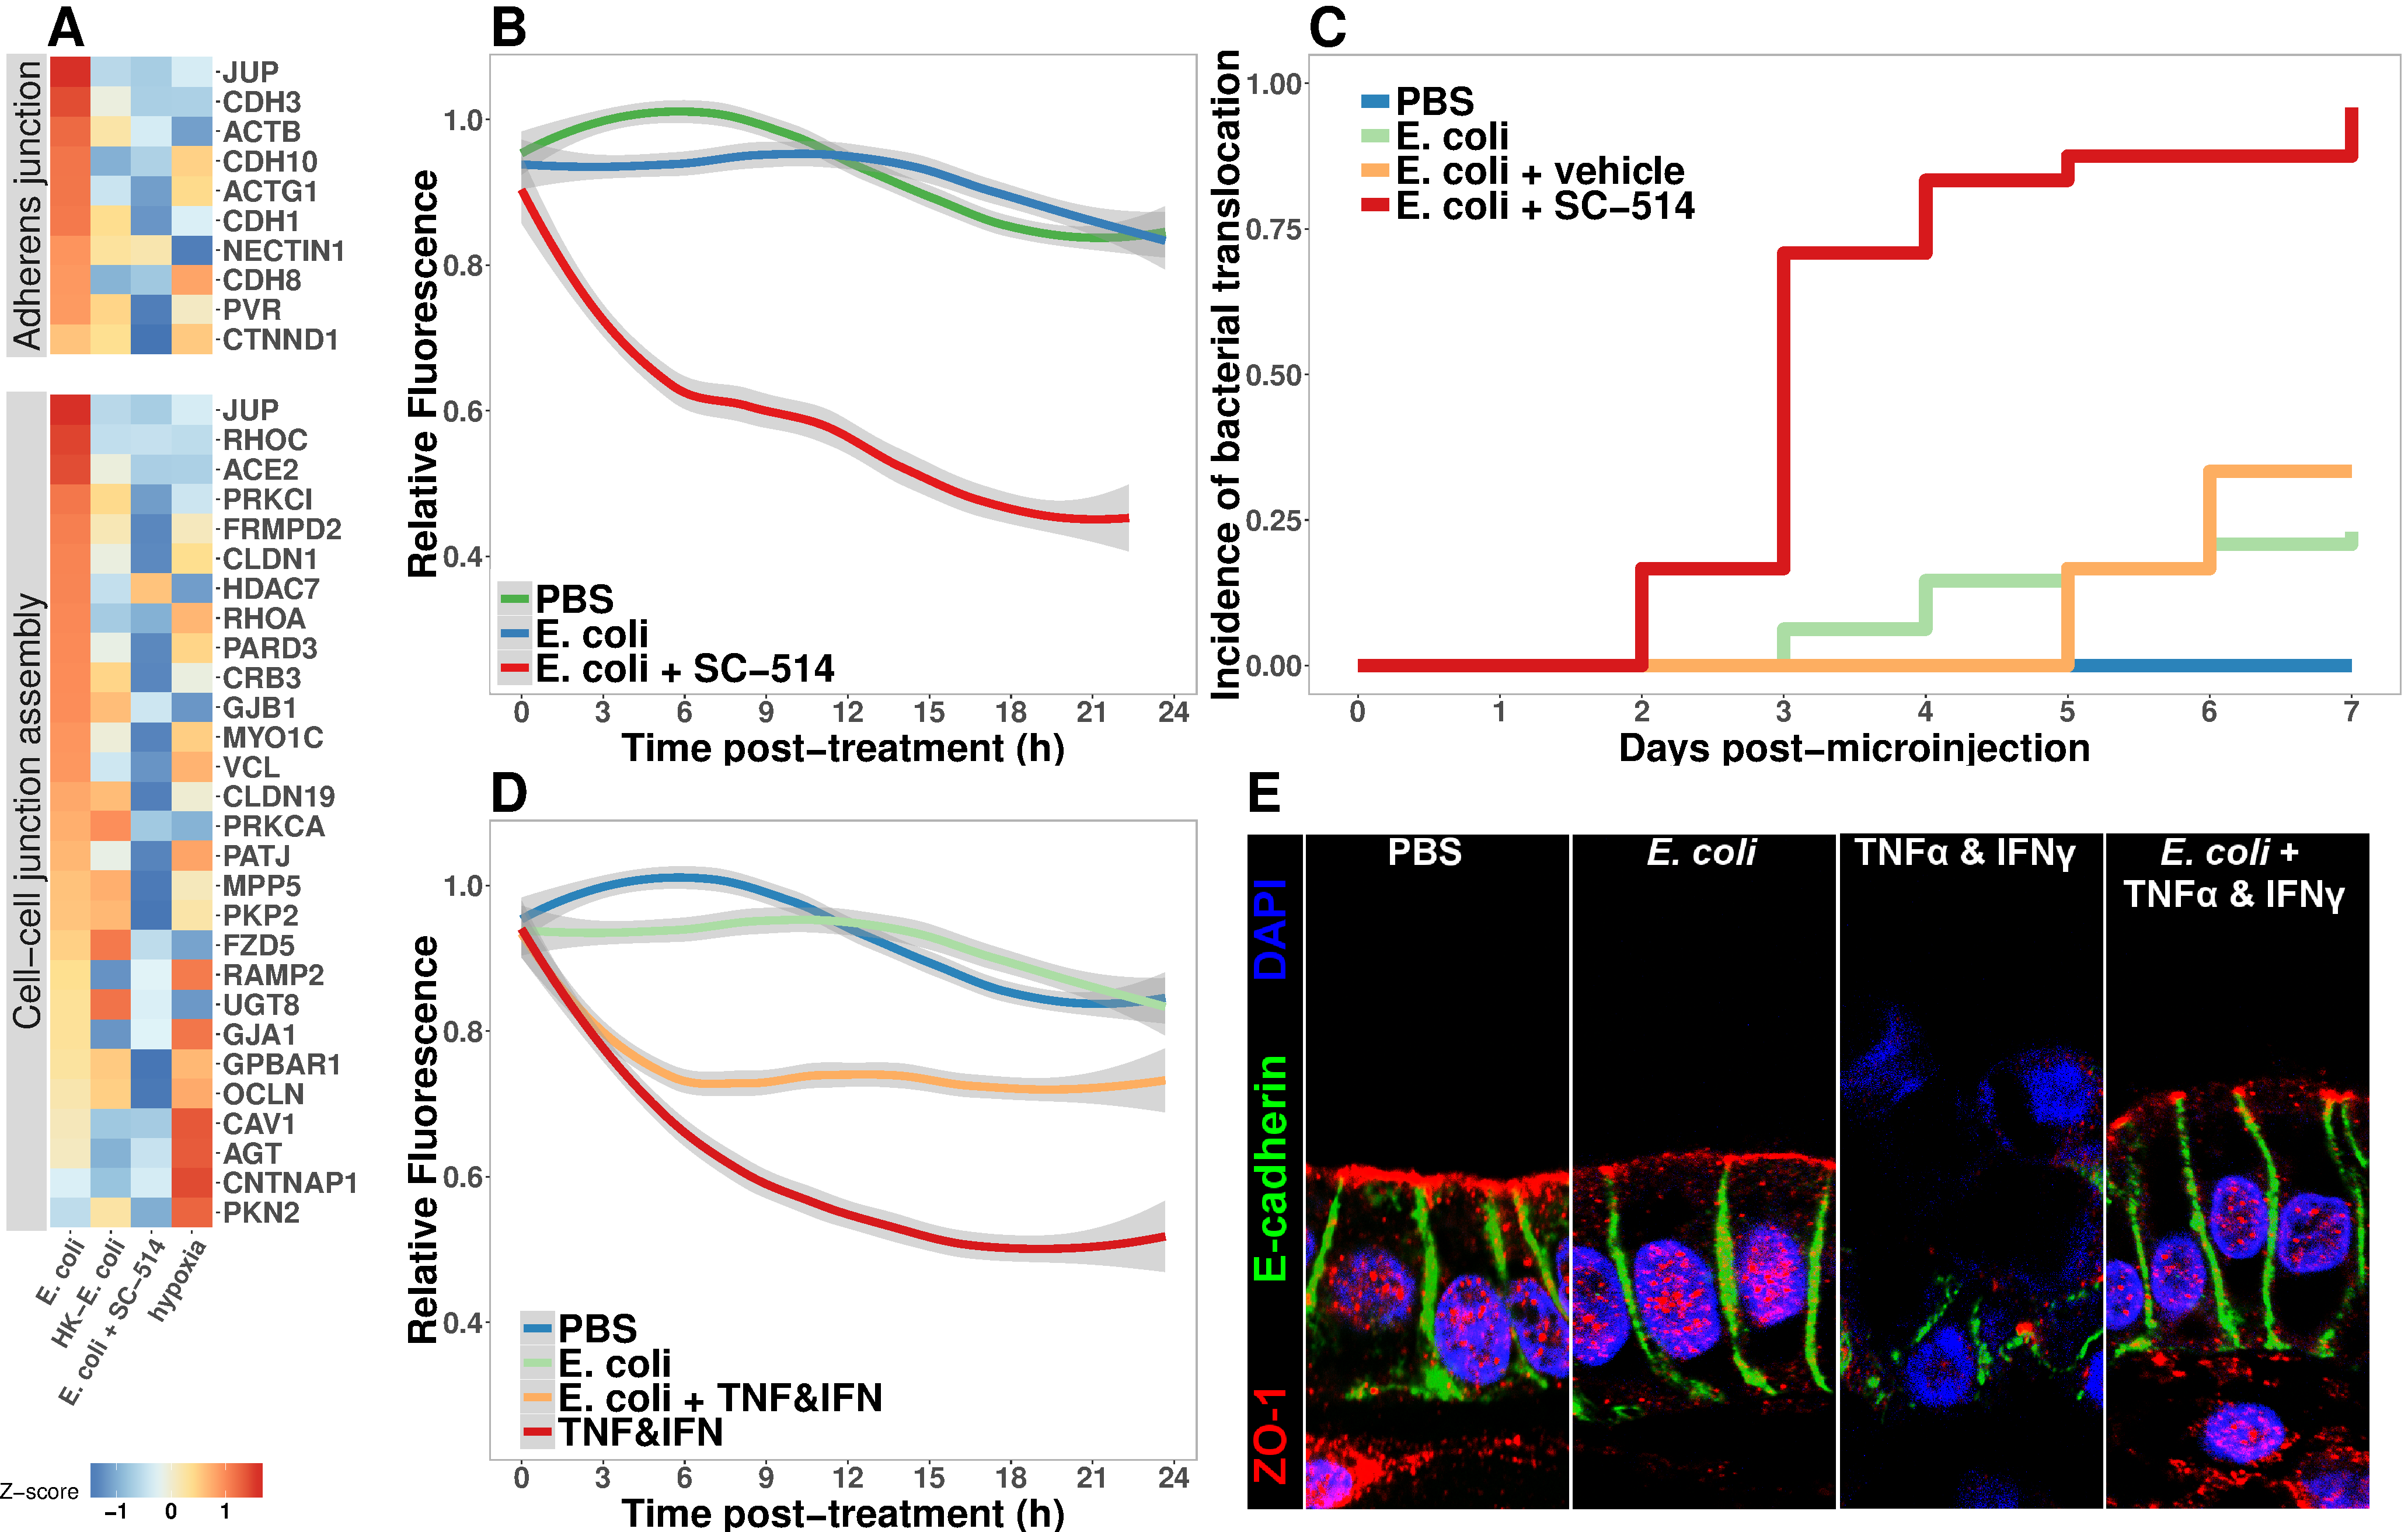
\includegraphics[width=0.95\linewidth]{./figures/figure7/figure7_multipanel.pdf}
\caption{\textbf{A} Heatmap of RNA-seq data indicating the relative expression of genes associated with the Adherens junction or Cell-cell junction assembly based on annotation in the REACTOME database. \textbf{B} Relative fluoresscence intensity over time in HIOs microinjected with 4 kDa FITC-dextran and imaged at 10 minute intervals. Line represents the best fit to the mean fluorescent intensity values in each condition with the grey region indicating S.E. for the fit line. N = 7-9 HIOs per group. \textbf{C} Rate of bacterial translocation over time in HIOs treated as indicated in the figure legend as detected by daily collection of external HIO media and enrichment in bacterial growth broth. N = 24 (\textit{E. coli} + SC-514) and N = 48 (\textit{E. coli}). \textbf{D} Relative fluoresscence intensity over time in HIOs microinjected with 4 kDa FITC-dextran and imaged at 10 minute intervals. Line represents the best fit to the mean fluorescent intensity values in each condition with the grey region indicating S.E. for the fit line. N = 8-9 HIOs per group. \textbf{E} Representative confocal micrographs of HIOs treated as indicated in D. Fluorescent immunostaining pseudocoloring applied as indicated in the figure legend. 60X optical magnification with 2X digital zoom. SC-514, small molecule inhibitor of NF-$\kappa$B ; HK, heat-inactivated; TNF, tumor necrosis factor-$\alpha$; IFN, interferon-$\gamma$}
\label{fig:fullwidth}
\end{fullwidth}
\end{figure}

\section*{{\bfseries\sffamily } Discussion}
\label{sec:orgheadline11}
The work presented here demonstrates that HIOs represent a robust model system to study the initial interactions between the gastrointestinal epithelium and colonizing microbes that occurs in the immediate postnatal period. Microorganisms introduced into the digestive tract at birth establish an intimate and mutualistic relationship with the host over time \citep{Costello:2012,Palmer:2007,Koenig:2011,Backhed:2015,Wopereis:2014}. However, the expansion of bacterial populations in the gut also presents a major challenge to intestinal homeostasis through the exposure to potentially inflammatory MAMPs \citep{Tanner:2015,Renz:2012}, consumption of tissue oxygen \citep{Glover:2016,Espey:2013,Albenberg:2014}, digestion of the mucus barrier \citep{Marcobal:2013,Desai:2016}, and competition for metabolic substrates \citep{Rivera-Chavez:2016,Kaiko:2016}. The mature intestinal epithelium serves as a crucial barrier to microbes that inhabit the lumen and mucosal surfaces \citep{Artis:2008,Turner:2009,Desai:2016,Kelly:2015,Cornick:2015,Peterson:2014,Hackam:2013,Turner:2009}. The specific function of the epithelium in adapting to initial microbial colonization, independent of innate and adaptive immune systems, remains unclear due to the lack of appropriate model systems that recapitulate host-microbe mutualism. Clarifying the role of the epithelium in colonization of the digestive tract by microorganisms is essential to understanding the molecular basis of the stable host-microbe mutualism in the mature intestine.

To examine the establishment of host-microbe mutualism, we chose to examine the interaction between the immature epithelium of HIOs and a non-pathogenic strain of \emph{E. coli}. Enterobacteriaceae, including \emph{E. coli}, are abundant in the newborn gut \citep{Palmer:2007,Koenig:2011,Backhed:2015,Yassour:2016}. Several large-scale surveys of microbial composition have demonstrated that \emph{E. coli} are among the most prevalent and abundant organisms in stool samples from newborns \citep{Backhed:2015,Koenig:2011}, in meconium \citep{Gosalbes:2013}, and in uterine tissue \citep{Aagaard:2014}. Non-pathogenic \emph{E. coli} strains may represent ideal model organisms for examining the impact of bacterial colonization of the immature epithelium due to their prevalence in the neonatal population and relevance to natural colonization, extensive characterization, and ease of laboratory manipulation. Microinjection of non-pathogenic \emph{E. coli} into the lumen of HIOs resulted in stable, long-term co-cultures (\textbf{Figure 1}). \emph{E. coli} grows rapidly within the HIO lumen (\textbf{Figure 1}), reaching densities roughly comparable to populations found in the human small intestine \citep{Donaldson:2016} within 24 h. Furthermore, the HIO is able to sustain this internal microbial population for several days while retaining the integrity of the epithelial barrier (\textbf{Figure 1}). Implicit is this observation is the conclusion that immature epithelium, along with a loosely structured mesenchymal layer, is intrinsically capable of adapting to the challenges imposed by colonization with non-pathogenic gut bacteria. 

To more closely examine these epithelial adaptations of microbial colonization, we performed transcriptional analysis of this response. HIOs colonized by \emph{E. coli} exhibit widespread transcriptional activation of innate bacterial recognition pathways, including TLR signaling cascades and downstream mediators such as NF-\(\kappa\)B (\textbf{Figure 2}). Indirect stimuli resulting from microbial activity can also shape epithelial function \citep{Buffie:2013}, and the transcriptome of \emph{E. coli}-colonized HIOs reflects a cellular response to reduced oxygen availability (\textbf{Figure 2}). Reduction of luminal O\(_{\text{2}}\) concentration occurs in the neonatal gut \citep{Gruette:1965,Fisher:2013,Zheng:2015}, possibly as a result of the consumption of dissolved O\(_{\text{2}}\) by the anaerobic and facultative anaerobic bacteria that predominate in the intestinal microbiome in early life \citep{Espey:2013,Fanaro:2003,Favier:2002,Palmer:2007}. We measured luminal oxygen content and epithelial hypoxia in HIOs microinjected with live \emph{E. coli}, finding that luminal oxygen concentration is reduced more than 10-fold relative to the surrounding media. This state of relative hypoxia extends into the epithelium itself and is correlated with increased microbial density (\textbf{Figure 3}). Thus, \emph{E. coli}-colonized HIOs recapitulate \emph{in vitro} the low-oxygen microenvironment found in the intestine.

Colonization of the HIO by \emph{E. coli} therefore comprises two broad stimuli: immediate exposure to contact-mediated signals such as MAMPs, and the onset of limiting luminal oxygen and epithelial hypoxia. Although the potential significance of exposure to microbial products in the context of tissue hypoxia is widely recognized in the setting of necrotizing enterocolitis \citep{Tanner:2015,Afrazi:2014,Hackam:2013,Neu:2011,Upperman:2005,Nanthakumar:2011}, this two factor signaling paradigm has not been well studied as a component of normal intestinal colonization and development. Using the HIO model system, it was possible to design experiments which separately examine the relative impact of microbial contact-mediated signals from microbe-associated hypoxic signals (\textbf{Figure 4}). This approach reveals that the full transcriptional response generated by the HIO following \emph{E. coli} colonization is the product of both contact-dependent and hypoxia-dependent signals, with heat-inactivated \emph{E. coli} or hypoxia alone recapitulating distinct subsets of the changes in gene expression observed in HIOs colonized with live \emph{E. coli} (\textbf{Figure 4}). NF-\(\kappa\)B signaling has been implicated in the downstream response to both microbial contact-mediated signals \citep{Zhang:2001,Xiao:2005,Kawai:2007} and tissue hypoxia \citep{Rius:2008,Arias-Loste:2015,Oliver:2009,Zeitouni:2016,Colgan:2013,Grenz:2012}. Pharmacologic inhibition of NF-\(\kappa\)B resulted in the suppression of both microbial contact- and hypoxia-associated gene expression in HIOs, inhibiting both contact-mediated epithelial barrier defense pathways and hypoxia-associated immune activation (\textbf{Figure 4}). NF-\(\kappa\)B appears to play a key role in integrating the complex stimuli resulting from exposure to microbial products and the onset of localized hypoxia in the immature intestinal epithelium during bacterial colonization.

The molecular and cellular maturation of the intestine that occurs during infancy ultimately results in enhanced functional capacity \citep{Lebenthal:1999,sanderson2000development,Neu:2007}. Bacterial colonization is associated with enhanced epithelial barrier function in gnotobiotic animals, including changes in the production of antimicrobial peptides and mucus \citep{Vaishnava:2008,Cash:2006,Goto:2014,Garcia-Lafuente:2001,Malago:2015,Menard:2008}. Defensins produced in the intestinal epithelium are critical mediators of the density and composition of microbial populations in the gut and protect the epithelium from microbial invasion \citep{Ostaff:2013,Cullen:2015,Salzman:2003,Salzman:2010}. Production of BD-2 is dramatically increased in HIOs immediately following \emph{E. coli} colonization (\textbf{Figures 2} and \textbf{5}), reaching concentrations that are sufficient to limit growth of \emph{E. coli} (\textbf{Figure 5}). Secreted and cell-surface associated mucins form a physical barrier to microbes in the gut, act as local reservoirs of antimicrobial peptide, and serve as substrates for the growth of beneficial microorganisms \citep{Desai:2016,Johansson:2016,Cornick:2015,Hansson:2012,Li:2015,Dupont:2014,Bergstrom:2013}. The immature HIO epithelium produces a robust mucus layer consisting of both neutral and acidic oligosaccharides with terminal carbohydrate modifications following colonization with \emph{E. coli} (\textbf{Figure 6}). Importantly, hypoxia alone does not result in the production of mucus while the introduction of heat-inactivated \emph{E. coli} induces mucus secretion at the apical epithelium (\textbf{Figure 6}), suggesting that microbial contact is the major stimulus eliciting mucus secretion in HIOs.

Epithelial barrier permeability is an important parameter of intestinal function reflecting the degree of selectivity in the transfer of nutrients across the epithelial layer and the exclusion of bacteria and other potentially harmful materials \citep{Bischoff:2014}. Increases in epithelial barrier permeability occur in the setting of inflammation \citep{Ahmad:2017,Michielan:2015} and infectious disease \citep{Shawki:2017}. Colonization of HIOs with \emph{E. coli} results in increased transcription of genes associated with the formation of the adherens junction and other cell-cell interactions in the epithelium (\textbf{Figure 7}). However, inhibition of NF-\(\kappa\)B signaling dramatically increases both epithelial barrier permeability and the rate of bacterial translocation (\textbf{Figure 7}), suggesting that NF-\(\kappa\)B signaling is critical to maintaining epithelial barrier integrity following colonization. Expression of genes involved in the formation of the cell junction and the production of antimicrobial defensins and mucus are NF-\(\kappa\)B dependent (\textbf{Figures 5-7}, \textbf{Figure 6 - Supplement 1},  \citealt{Tsutsumi-Ishii:2002,Ahn:2005}). The inability to mount an effective innate defense response in the presence of NF-\(\kappa\)B inhibition results in the failure of the HIO epithelial barrier and the loss of co-culture stability (\textbf{Figure 7}). This result underscores the critical role of NF-\(\kappa\)B signaling in the formation of a stable host-microbe mutualism at the immature epithelial interface.

Dysregulated production of pro-inflammatory cytokines  contributes to the loss of epithelial barrier integrity in NEC \citep{Tanner:2015,Hackam:2013,Neu:2011,Nanthakumar:2011,Halpern:2003,Ford:1997,Ford:1996,Tan:1993}; this is recapitulated in HIOs, as exposure to pro-inflammatory cytokines results in the rapid loss of epithelial barrier integrity and the dissolution of epithelial tight junctions (\textbf{Figure 7}). Probiotics may promote epithelial barrier integrity in NEC \citep{Robinson:2014,Alfaleh:2011,Underwood:2014,Khailova:2009} and HIOs colonized by \emph{E. coli} exhibit enhanced epithelial barrier resilience (\textbf{Figure 7}). Functional maturation resulting from colonization of the immature intestinal epithelium may therefore play an essential role in promoting the resolution of physiologic inflammation.

While great progress has been made in characterizing the composition of the gut microbiota in health and disease \citep{Shreiner:2015,Costello:2012}, this approach has a limited ability to discern the contributions of individual bacteria to the establishment of host-microbe symbiosis. Our work establishes an approach that recapitulates host-microbe mutualism in the immature human intestine in an experimentally tractable \emph{in vitro} model system. Application of this approach may facilitate the development of mechanistic models of host-microbe interactions in human tissue in health and disease. For example, one of the major limitations in our understanding of NEC has been the lack of an appropriate model system to study colonization of the immature intestine \citep{Neu:2011,Balimane:2005,Tanner:2015,Nguyen:2015}. Our results suggest that colonization of the HIO with a non-pathogenic gut bacteria results in functional maturation of the epithelial barrier. Future work which examines the effects of organisms associated with the premature gut \citep{Morrow:2013,Greenwood:2014,Ward:2016} on the molecular, cellular, and functional maturation of the immature epithelium may be instrumental in elucidating mechanisms of microbiota-associated disease pathogenesis in the immature intestine.

\section*{{\bfseries\sffamily } Materials and Methods}
\label{sec:orgheadline25}

\subsection*{{\bfseries\sffamily } HIO culture}
\label{sec:orgheadline12}
Human ES cell line  H9 (NIH registry \#0062) was obtained from the WiCell Research Institute. Stem cells were maintained on Matrigel (BD Biosciences, San Jose, CA) in mTeSR1 medium (STEMCELL Technologies, Vancouver, Canada). hESCs were passaged and differentiated into human intestinal organoid tissue as previously described \citep{Spence:2011,McCracken:2011}. HIOs were maintained in ENR media without antibiotics prior to microinjection experiments.
For hypoxic culture experiments, HIOs were transferred to a hydrated and sealed Modular Incubator Chamber (MIC-101, Billups-Rothenburg, Inc. Del Mar CA) filled with 1\% O\(_{\text{2}}\), 5\% CO\(_{\text{2}}\), and balance N\(_{\text{2}}\) and maintained at \SI{37}{\celsius} for 24 h.
\subsection*{{\bfseries\sffamily } HIO transplantation and tissue derived enteroid culture}
\label{sec:orgheadline13}
HIO transplantations: This study was performed in strict accordance with the recommendations in the Guide for the Care and Use of Laboratory Animals of the National Institutes of Health. All animal experiments were approved by the University of Michigan Institutional Animal Care and Use Committee (IACUC; protocol \# PRO00006609). HIO transplants into the kidney capsule were performed as previously described \citep{Finkbeiner:2015,Dye:2016} Briefly, mice were anesthetized using 2\% isofluorane. The left flank was sterilized using Chlorhexidine and isopropyl alcohol, and an incision was made to expose the kidney. HIOs were manually placed in a subcapsular pocket of the kidney of male 7–10 week old NOD-SCID IL2Rgnull (NSG) mice using forceps. An intraperitoneal flush of Zosyn (100 mg/kg; Pfizer Inc.) was administered prior to closure in two layers. The mice were sacrificed and transplant retrieved after 10 weeks. 
Human Tissue: Normal, de-identified human fetal intestinal tissue was obtained from the University of Washington Laboratory of Developmental Biology. Normal, de-identified human adult intestinal tissue was obtained from deceased organ donors through the Gift of Life, Michigan. All human tissue used in this work was obtained from non-living donors, was de-identified and was conducted with approval from the University of Michigan IRB (protocol \# HUM00093465 and HUM00105750).  Isolation and culture of HIO epithelium, transplanted HIO epithelium, fetal and adult human duodenal epithelium was carried out as previously described \citep{Finkbeiner:2015}, and was cultured in a droplet of Matrigel using L-WRN conditioned medium to stimulate epithelial growth, as previously described \citep{Miyoshi:2012,Miyoshi:2013}
\subsection*{{\bfseries\sffamily } Bacterial culture}
\label{sec:orgheadline14}
\emph{Escherichia coli} strain ECOR2 (ATCC 35321) was cultured in Lysogeny broth media or 1.5\% agar plates at \SI{37}{\celsius} under atmospheric oxygen conditions. Glycerol stock solutions are available upon request. 
\subsection*{{\bfseries\sffamily } Microinjection}
\label{sec:orgheadline15}
Microinjections were performed using a protocol modified from \citet{Leslie:2015}. Briefly, HIOs were injected using thin wall glass capillaries (TW100F-4, World Precision Instruments, Sarasota FL) shaped using a P-30 micropipette puller (Sutter Instruments, Novato CA). Pulled microcapilaries were mounted on a Xenoworks micropipette holder with analog tubing (BR-MH2 \& BR-AT, Sutter Instruments) attached to a 10 ml glass syringe filled with sterile mineral oil (Fisher Scientific, Hampton NH). Fine control of the micropippette was achieved using a micromanipulator (Narishge International Inc., East Meadow NY) and microinjection was completed under 1-2X magnification on an SX61 stereo dissecting scope (Olympus, Tokyo Japan). HIOs suspended in Matrigel (Corning Inc., Corning NY) were injected with approximately 1 \(\mu\)l solution. In bacterial microinjection experiments, the HIO culture media was removed immediately following microinjection and the cultures were rinsed with PBS and treated with ENR media containing penicillin and streptomycin to remove any bacteria introduced to the culture media during the microinjection process. After 1 h at \SI{37}{\celsius}, the media was replaced with fresh anti-biotic free ENR.
\subsection*{{\bfseries\sffamily } Measurement of luminal oxygen}
\label{sec:orgheadline16}
Luminal oxygen content was measured in HIOs using an optically coated implantable microsensor with a tip tapered at < 50 \(\mu\)m (IMP-PSt1, PreSens Precision Sensing GmbH) attached to a micro fiber optic oxygen meter (Microx TX3, PreSens Precision Sensing GmbH, Regensburg Germany). The oxygen probe was calibrated according to the manufacturer's instructions and measurements of the external media and HIO luminal oxygen content were collected by mounting the microsensor on a micromanipulator (Narishge International Inc., East Meadow NY) and guiding the sensor tip into position using 1-2X magnification on a stereo dissecting scope (Olympus, Tokyo Japan). All oxygen concentration readings were analyzed using PreSens Oxygen Calculator software (TX3v531, PreSens Precision Sensing GmbH, Regensburg Germany). 
For measurement of relative cytoplasmic hypoxia, HIO cultures were treated with 100 \(\mu\)M pimonidazol HCl (Hypoxyprobe, Inc., Burlington MA) added to the external culture media and incubated at \SI{37}{\celsius} and 5\% CO\(_{\text{2}}\) for 2 h prior to fixation in 4\% parafomaldehyde. Pimonidazole conjugates were stained in tissue sections using the Hypoxyprobe-1 mouse IgG monoclonal antibody (Hypoxyprobe, Inc., Burlington MA) with appropriate secondary antibody (see antibody dilutions table).
\subsection*{{\bfseries\sffamily } Immunohistochemistry}
\label{sec:orgheadline17}
Immunostaining was carried out as previously described \citep{Finkbeiner:2015}. Antibody information and dilutions can be found in \textbf{Supplementary File 3}. All images were taken on a Nikon A1 confocal microscope or an Olympus IX71 epifluorescent microscope. CarboFree blocking buffer (SP-5040; Vector Laboratories, Inc. Burlingame CA) was substituted for dilute donkey serum in PBS in staining for mucins and carbohydrate moieties.
\subsection*{{\bfseries\sffamily } NF-\(\kappa\)B inhibition}
\label{sec:orgheadline18}
The NF-\(\kappa\)B inhibitor SC-514 \citep{Kishore:2003,Litvak:2009} (Tocris Cookson, Bristol, United Kingdom) was re-suspended in DMSO at a concentration of 25 mM. HIOs were treated with SC-514 suspended in DMSO added to the external ENR culture media at a final concentration of 1 \(\mu\)M. Efficacy of SC-514 was verified by Western blot of lysates from HIOs injected with PBS or live \emph{E. coli} or injected with live \emph{E. coli} in the presence of 1 \(\mu\)M SC-514 added to the external media. HIOs were collected after 24 hours in lysis buffer composed of 300 mM NaCl, 50mM Tris base, 1mM EDTA, 10\% glycerol, 0.5\% NP-40, and 1X Halt Phosphatase Inhibitor Cocktail (Pierce Biotechnology, Rockford IL). Lysates were separated on a 10\% Bis-Tris polyacrylamide gel under reducing conditions (Invitrogen, Carlsbad CA) and transferred to PVDF using a wet transfer apparatus (Bio-Rad Laboratories, Hercules CA) overnight at \SI{4}{\celsius}. The PVDF membrane was blocked in Odyssey TBS blocking buffer (LI-COR Biosciences, Lincoln NE). The membrane was submerged in blocking buffer containing primary rabbit monoclonal antibodies against phosphorylated NF-\(\kappa\)B p65 (1:200, Cell Signaling Technology \#3033S) or total NF-\(\kappa\)B p65 (1:400, Cell Signaling Technology \#8242S) and incubated at room temperature for 2 h. All washes were conducted in Tris-buffered saline with 1\% Tween-20 (TBST). The secondary goat anti-rabbit IgG IRDye 800CW was diluted 1:15,000 in TBST and exposed to the washed membrane for 1 h at room temperature. After additional washes, the PVDF membrane was imaged using an Odyssey Scanner (LI-COR Biosciences, Lincoln NE).
\subsection*{{\bfseries\sffamily } Bacterial translocation assay}
\label{sec:orgheadline19}
Incidence of bacterial translocation was determined in HIOs plated individually in single wells of 24-well plates and microinjected with \emph{E. coli}. The external culture media was collected and replaced daily. The collected media was diluted 1:10 in LB broth in 96 well plates and cultured at \SI{37}{\celsius} overnight. Optical density (600 nm) was measured in the 96-well LB broth cultures using a VersaMax microplate reader (Molecular Devices, LLC, Sunnyvale CA). OD\(_{\text{600}}\) > sterile LB broth baseline was considered a positive culture. 
\subsection*{{\bfseries\sffamily } FITC-dextran permeability}
\label{sec:orgheadline20}
For epithelial permeability assays, HIOs were microinjected with 4 kDa FITC-dextran suspended in PBS at a concentration of 2 mg/ml as described previously \citep{Leslie:2015} using the microinjection system detailed above. Images were collected at 10 minute intervals at 4X magnification on an Olympus IX71 epifluorescent microscope using a Deltavision RT live cell imaging system with Applied Precision softWoRx imaging software (GE Healthcare Bio-Sciences, Marlborough MA). Cultures were maintained at \SI{37}{\celsius} and 5\% CO\(_{\text{2}}\) throughout the imaging timecourse. For experiments involving cytokine treatment, recombinant TNF-\(\alpha\) and INF-\(\gamma\) were added to the external culture media at a concentration of 500 ng/ml at the start of the experiment.
\subsection*{{\bfseries\sffamily } \emph{In vitro} antimicrobial activity assay}
\label{sec:orgheadline21}
Recombinant human BD-2 (Abcam, Cambridge MA) was reconstituted in sterile LB broth and diluted to 0.1-1 \(\mu\)g/ml. \emph{E. coli} cultures were diluted 1:1000 in sterile LB containing 0-1 \(\mu\)/ml BD-2 and transferred to a 96-well microplate. A VersaMax microplate reader (Molecular Devices, LLC, Sunnyvale CA) was used to measure OD\(_{\text{600}}\) at 10 minute intervals in microplates maintained at \SI{37}{\celsius} with regular shaking  over a 18 h timecourse.
\subsection*{{\bfseries\sffamily } ELISA assays}
\label{sec:orgheadline22}
Secreted cytokine, antimicrobial peptide, and growth factor concentrations were determined by ELISA (Duosets, R\&D Systems, Minneapolis, MN) using the manufacturer's recommended procedures at the Immunological Monitoring Core of the University of Michigan Cancer Center.
\subsection*{{\bfseries\sffamily } RNA sequencing and analysis}
\label{sec:orgheadline23}
RNA was isolated using the mirVana RNA isolation kit and following the "Total RNA" isolation protocol (Thermo-Fisher Scientific, Waltham MA). RNA library preparation and RNA-sequencing (single-end, 50 bp read length) were performed by the University of Michigan DNA Sequencing Core using the Illumina Hi-Seq 2500 platform. All sequences were deposited in the EMBL-EBI ArrayExpress database using Annotare 2.0 and are cataloged under the accession number \textbf{E-MTAB-5801}. Transcriptional quantitation analysis was conducted using 64-bit Debian Linux stable version 7.10 ("Wheezy"). Pseudoalignment of RNA-seq data was computed using kallisto v0.43.0 \citep{Bray:2016} and differential expression of pseudoaligned sequences was calculated using the R package DEseq2 \citep{Love:2014}.
\subsection*{{\bfseries\sffamily } Statistical analysis}
\label{sec:orgheadline24}
Unless otherwise indicated in the figure legends, differences between experimental groups or conditions were evaluated using an unpaired Student's \emph{t}-test. A \emph{P}-value < 0.05 was considered to represent a statistically significant result. All statistical analyses were conducted using R version 3.4.0 (2017-04-21) \citep{CRAN:2017} and plots were generated using the R package ggplot2 \citep{Wickham:2009}. Gene pathway over-representation tests and Gene Set Enrichment Analysis \citep{Subramanian:2005} were implemented using the R packages clusterProfiler \citep{Yu:2012} and ReactomePA \citep{Yu:2016}. Analyses conducted in R were collated and using Emacs v25.2 \citep{Stallman:1981:EEC:1159890.806466} with Org-mode v8.3.5 and the paper was written in \LaTeX{} using Emacs. Complete analysis scripts are available at \url{https://github.com/hilldr/Hill_HIO_Colonization_2017}.
\section*{{\bfseries\sffamily } Acknowledgments}
\label{sec:orgheadline26}
The authors would like to thank Joel Whitfield of the Immunological Monitoring Core of the University of Michigan Cancer Center, Robert Lyons and Tricia Tamsen of the University of Michigan DNA Sequencing Core, and Chris Edwards of the University of Michigan Molecular Imaging Laboratory for invaluable technical assistance.
JRS is supported by the Intestinal Stem Cell Consortium (U01DK103141), a collaborative research project funded by the National Institute of Diabetes and Digestive and Kidney Diseases (NIDDK) and the National Institute of Allergy and Infectious Diseases (NIAID), and by the NIAID Novel, Alternative Model Systems for Enteric Diseases (NAMSED) consortium (U19AI116482). DRH is supported the Mechanisms of Microbial Pathogenesis training grant from the National Institute of Allergy and Infectious Disease (NIAID, T32AI007528) and the Clinical and Translational Science award to the Michigan Institute for Clinical and Health Research (UL1TR000433). 
\bibliography{bibliography.bib}
\nocite{*}
\end{document}